\documentclass{article}
\usepackage{iclr2026_conference,times}

\input{math_commands.tex}

\usepackage{hyperref}
\usepackage{url}
\usepackage{booktabs}
\usepackage{multirow}
\usepackage{graphicx}
\usepackage{subcaption}

\begin{document}

\title{Do Large Language Models Develop Moral Reasoning Stages? \\
An Empirical Analysis Using Kohlberg's Framework}

\author{Anonymous Authors}

\maketitle


% -----------------------------------------------------------------------
\begin{abstract}
% -----------------------------------------------------------------------

Understanding how moral reasoning capabilities develop in large language models (LLMs) is important for AI alignment, informs whether human developmental frameworks apply to artificial systems, and identifies when and how to introduce moral objectives during training. In this work, we investigate whether LLMs exhibit developmental progression in moral reasoning analogous to that observed in human cognition, specifically, whether model scale and alignment training produce systematic progression through Kohlberg's stages of moral development, or whether models instead learn to generate reasoning-\emph{like} outputs that superficially resemble mature moral judgment without the underlying developmental trajectory.

Using Kohlberg's theory of moral development as an analytical framework, we evaluate more than 600 responses generated by 13 modern LLMs spanning a range of architectures, parameter scales, and training regimes across six classical moral dilemmas. We propose an LLM-as-judge scoring pipeline that classifies each response into one of Kohlberg's six developmental stages and validate its reliability across multiple judge models. We conduct ten complementary analyses examining scale effects, prompting sensitivity, cross-dilemma consistency, human distributional comparisons, action--reasoning alignment, linguistic patterns, response quality, the independent contributions of scale and training, sub-capability thresholds, and stage transition dynamics.

Our results reveal a striking and consistent pattern: responses overwhelmingly correspond to post-conventional moral reasoning (Stages~5--6) regardless of model size, architecture, or prompting strategy: a distribution that is effectively the inverse of human developmental norms, where Stage~4 dominates. While factorial analysis confirms that model scale carries a statistically significant effect on mean stage ($F(2,229)=6.05$, $p=0.003$, $\eta^2=0.050$), the practical magnitude is small (Cohen's $d=0.55$, Large vs.\ Small) and insufficient to produce developmental differentiation: even the smallest evaluated models consistently produce post-conventional outputs. Training type shows no significant independent main effect ($p=0.065$), though reasoning-tuned models score higher than base-RLHF models within the large-scale group. Critically, models exhibit near-robotic cross-dilemma consistency (ICC~$>$~0.90), the inverse of human moral variability, and a subset show \emph{moral decoupling}: high-stage vocabulary paired with low-stage action choices. We posit that these patterns collectively constitute evidence for \emph{moral ventriloquism}: the acquisition, through alignment training, of the rhetorical conventions of mature moral reasoning without the underlying developmental trajectory those conventions are meant to represent.

\end{abstract}

\begin{figure}[t]
  \centering
  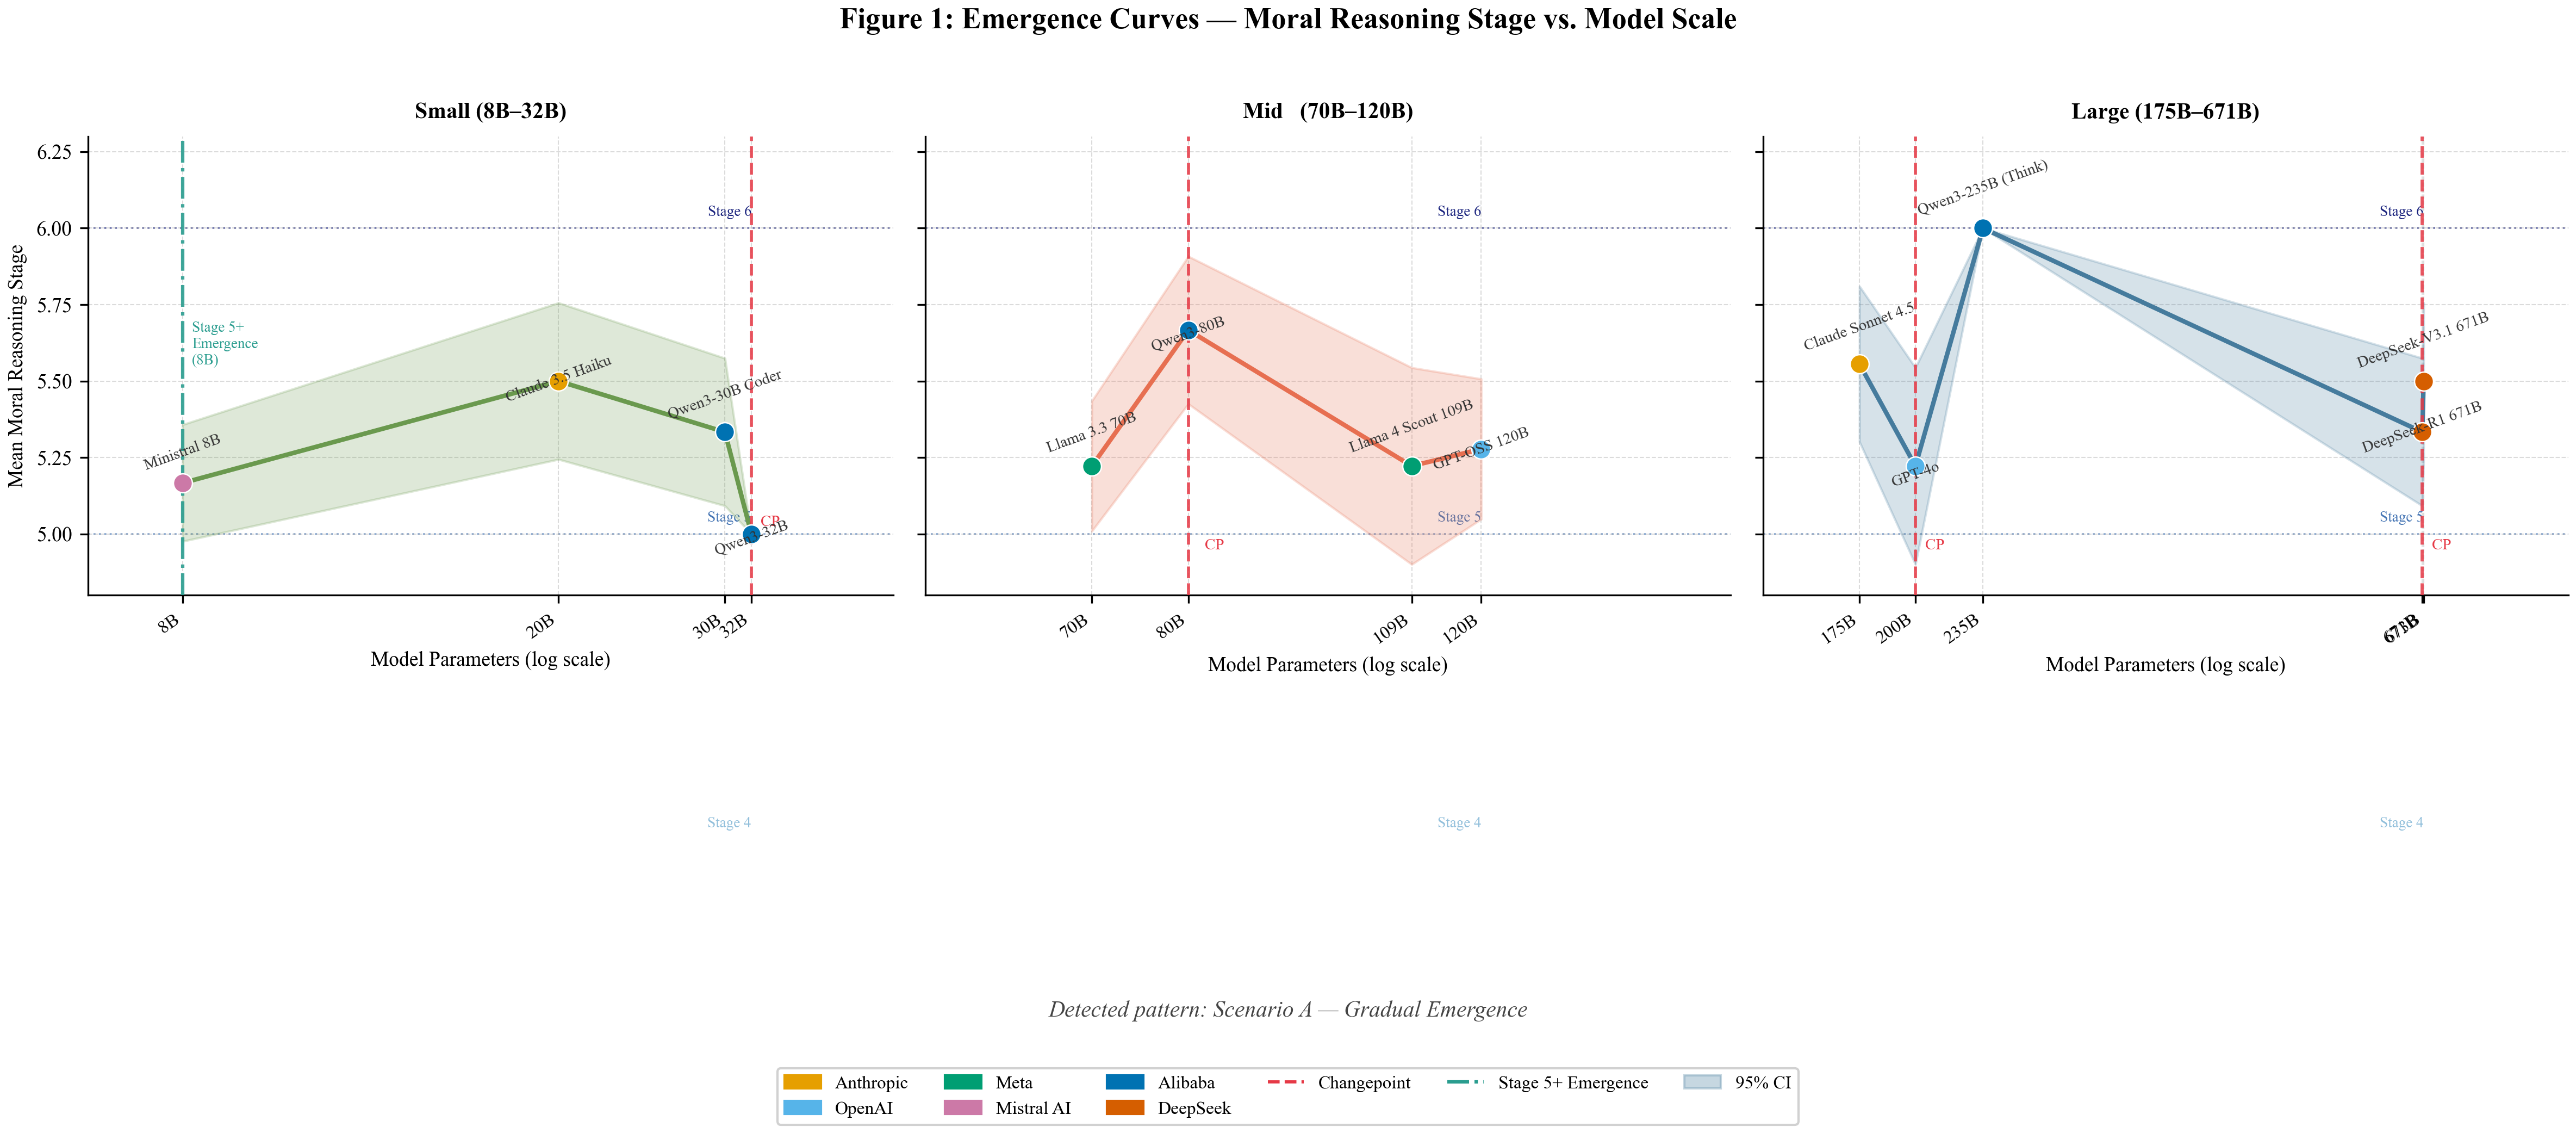
\includegraphics[width=\textwidth]{images/analysis7_fig1_emergence_curves.png}
  \caption{\textbf{Emergence of Post-Conventional Moral Reasoning Across Model Scale.} Stage emergence curves showing the proportion of post-conventional (Stages~5--6) responses as a function of model parameter count. Post-conventional outputs emerge at high rates even for the smallest evaluated models and plateau near ceiling across all scale tiers, indicating that the rhetorical register of mature moral reasoning is acquired early in the scaling regime rather than emerging gradually with capability growth.}
  \label{fig:heatmap_overview}
\end{figure}

% -----------------------------------------------------------------------
\section{Introduction}
% -----------------------------------------------------------------------

A central question in AI alignment is not just whether large language models (LLMs) produce morally acceptable outputs, but \emph{how} and \emph{when} moral reasoning capabilities develop during training. Understanding this question has direct practical consequences: it informs when to introduce moral objectives during training, reveals whether human developmental frameworks apply to artificial systems, and identifies capability thresholds at which models may be considered ready for deployment in ethically sensitive domains.

Modern LLMs frequently generate detailed, sophisticated-sounding explanations when confronted with moral dilemmas, invoking abstract principles such as human dignity, social contracts, and universal rights. These behaviors are often interpreted as evidence that models possess genuine moral reasoning capabilities. At the same time, a growing body of research has raised serious concerns about interpreting model outputs as evidence of genuine underlying processes. Several studies suggest that LLMs may produce convincing reasoning patterns through statistical pattern completion rather than through explicit reasoning mechanisms \citep{turpin2023language, chen2025reasoning}. In particular, recent work questions whether chain-of-thought explanations correspond to the internal computational processes that generate model predictions, or whether intermediate tokens instead reflect learned stylistic patterns associated with reasoning discourse \citep{kambhampati2024planllms}. These concerns raise an important challenge: if models can produce explanations that \emph{resemble} reasoning without performing the underlying reasoning processes, behavioral evaluations based solely on model outputs may provide a systematically misleading picture of model capability.

Moral reasoning provides a particularly informative setting in which to examine this question. Moral dilemmas typically involve competing principles, social norms, and abstract ethical concepts, requiring models to generate explanations that balance multiple constraints while appealing to broader normative frameworks. Crucially, if LLMs genuinely develop moral reasoning capabilities as a function of scale and training, we would expect their outputs to mirror the developmental trajectory observed in humans, varying across contexts, progressing with scale, and converging toward the Stage~4 distribution that characterizes most human adults, not clustering uniformly at the highest stages regardless of model size or training procedure.

In this work, we study moral reasoning in large language models using Kohlberg's theory of moral development as our evaluation framework. Kohlberg's framework categorizes moral reasoning into six stages reflecting increasing levels of abstraction and principle-based reasoning. Early stages (1--2) emphasize punishment avoidance and self-interest, middle stages (3--4) invoke social expectations and rule adherence, and later stages (5--6) appeal to abstract ethical principles such as human rights and social contracts. In human populations, most adults reason primarily at Stage~4, while Stage~6 reasoning, grounded in universal ethical principles, is comparatively rare. This known distribution provides a principled baseline against which model outputs can be evaluated diagnostically.

If LLMs develop increasingly sophisticated moral reasoning as model capabilities scale, we would expect to observe systematic variation in the stages of reasoning produced by different models: smaller models producing lower-stage reasoning and larger models producing more abstract, principle-based reasoning. However, if models instead learn to generate explanations that \emph{resemble} high-quality moral reasoning, particularly through alignment training that rewards socially acceptable outputs, we may observe a very different pattern: systematic generation of high-stage responses regardless of model size or architecture.

To investigate this question, we conduct a large-scale empirical study evaluating moral reasoning patterns across 13 state-of-the-art LLMs, conducting ten complementary quantitative analyses to characterize the nature, robustness, and internal coherence of these patterns. Figure~\ref{fig:intro_preview} previews two headline findings that shape our investigation. Our methodology is motivated by the following research questions:

\begin{description}
    \item[\textbf{RQ1}] Does model scale predict higher Kohlberg stage, and what is the effect size?
    \item[\textbf{RQ2}] Does prompting strategy systematically influence moral stage?
    \item[\textbf{RQ3}] Are model stage assignments consistent across dilemmas, and how does this compare to human moral variability?
    \item[\textbf{RQ4}] Do LLM stage distributions resemble human developmental norms?
    \item[\textbf{RQ5}] Do models practice what they preach: Does stated high-stage reasoning correspond to high-stage action choices?
    \item[\textbf{RQ6}] Does scale affect moral reasoning independent of training type, or does training dominate once scale is controlled?
\end{description}

\begin{figure}[h]
  \centering
  \begin{subfigure}[t]{0.48\textwidth}
    \centering
    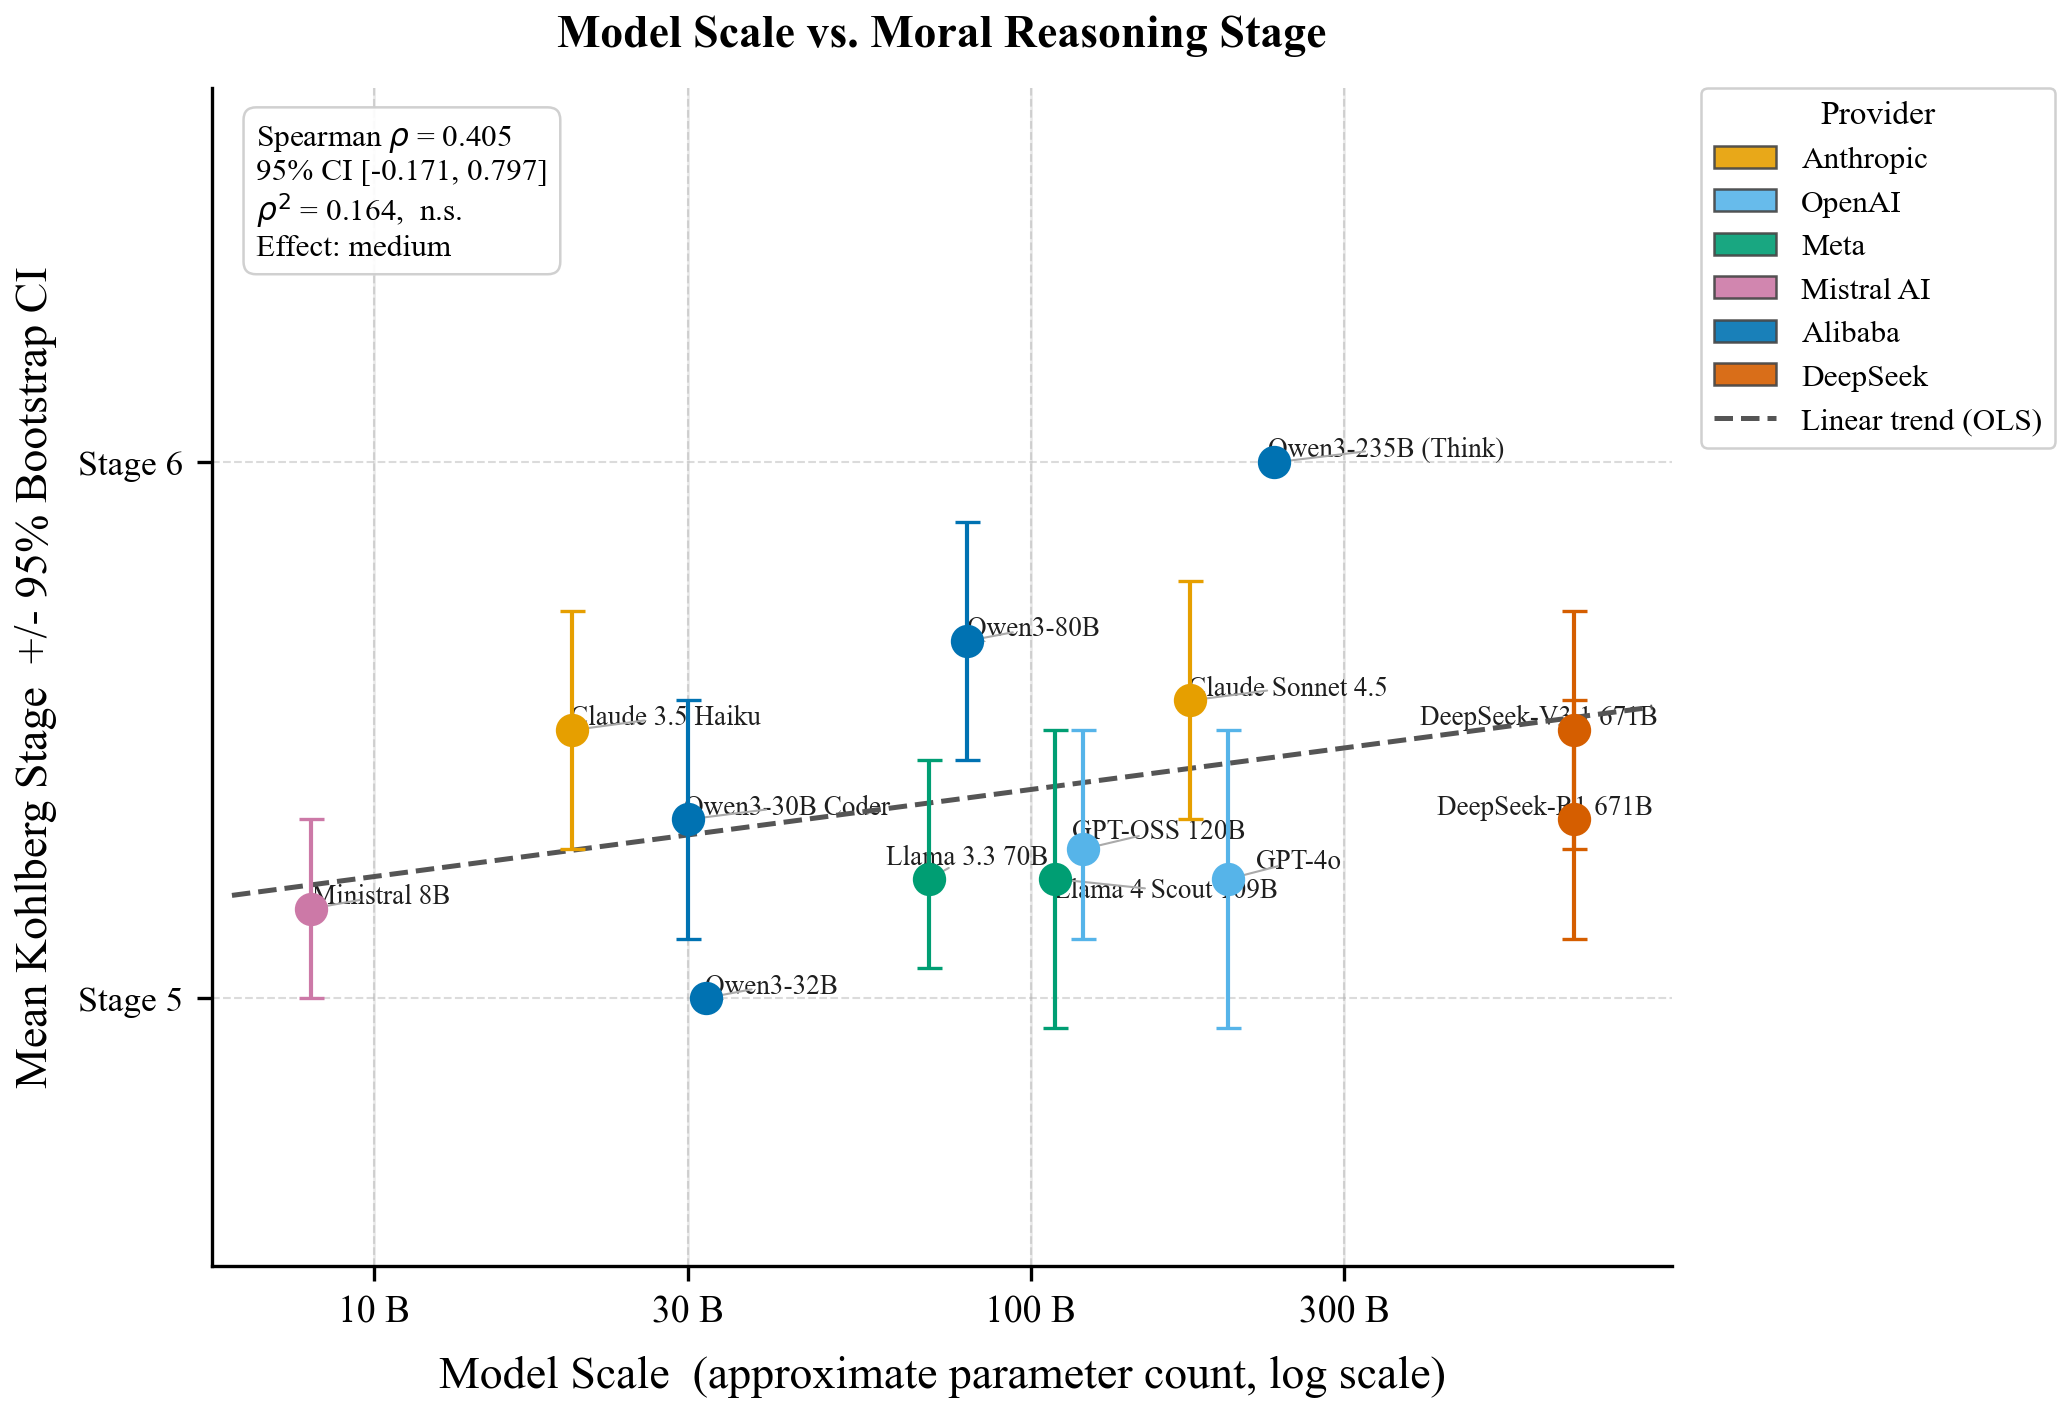
\includegraphics[width=\textwidth]{images/analysis1_fig2_scatter_scale_vs_stage.png}
    \caption{Scale vs.\ moral stage (Spearman $\rho=0.52$). Despite a statistically significant correlation, the entire range spans $<$1 stage point (5.00--6.00), and even the smallest model sits firmly in the post-conventional region.}
  \end{subfigure}\hfill
  \begin{subfigure}[t]{0.48\textwidth}
    \centering
    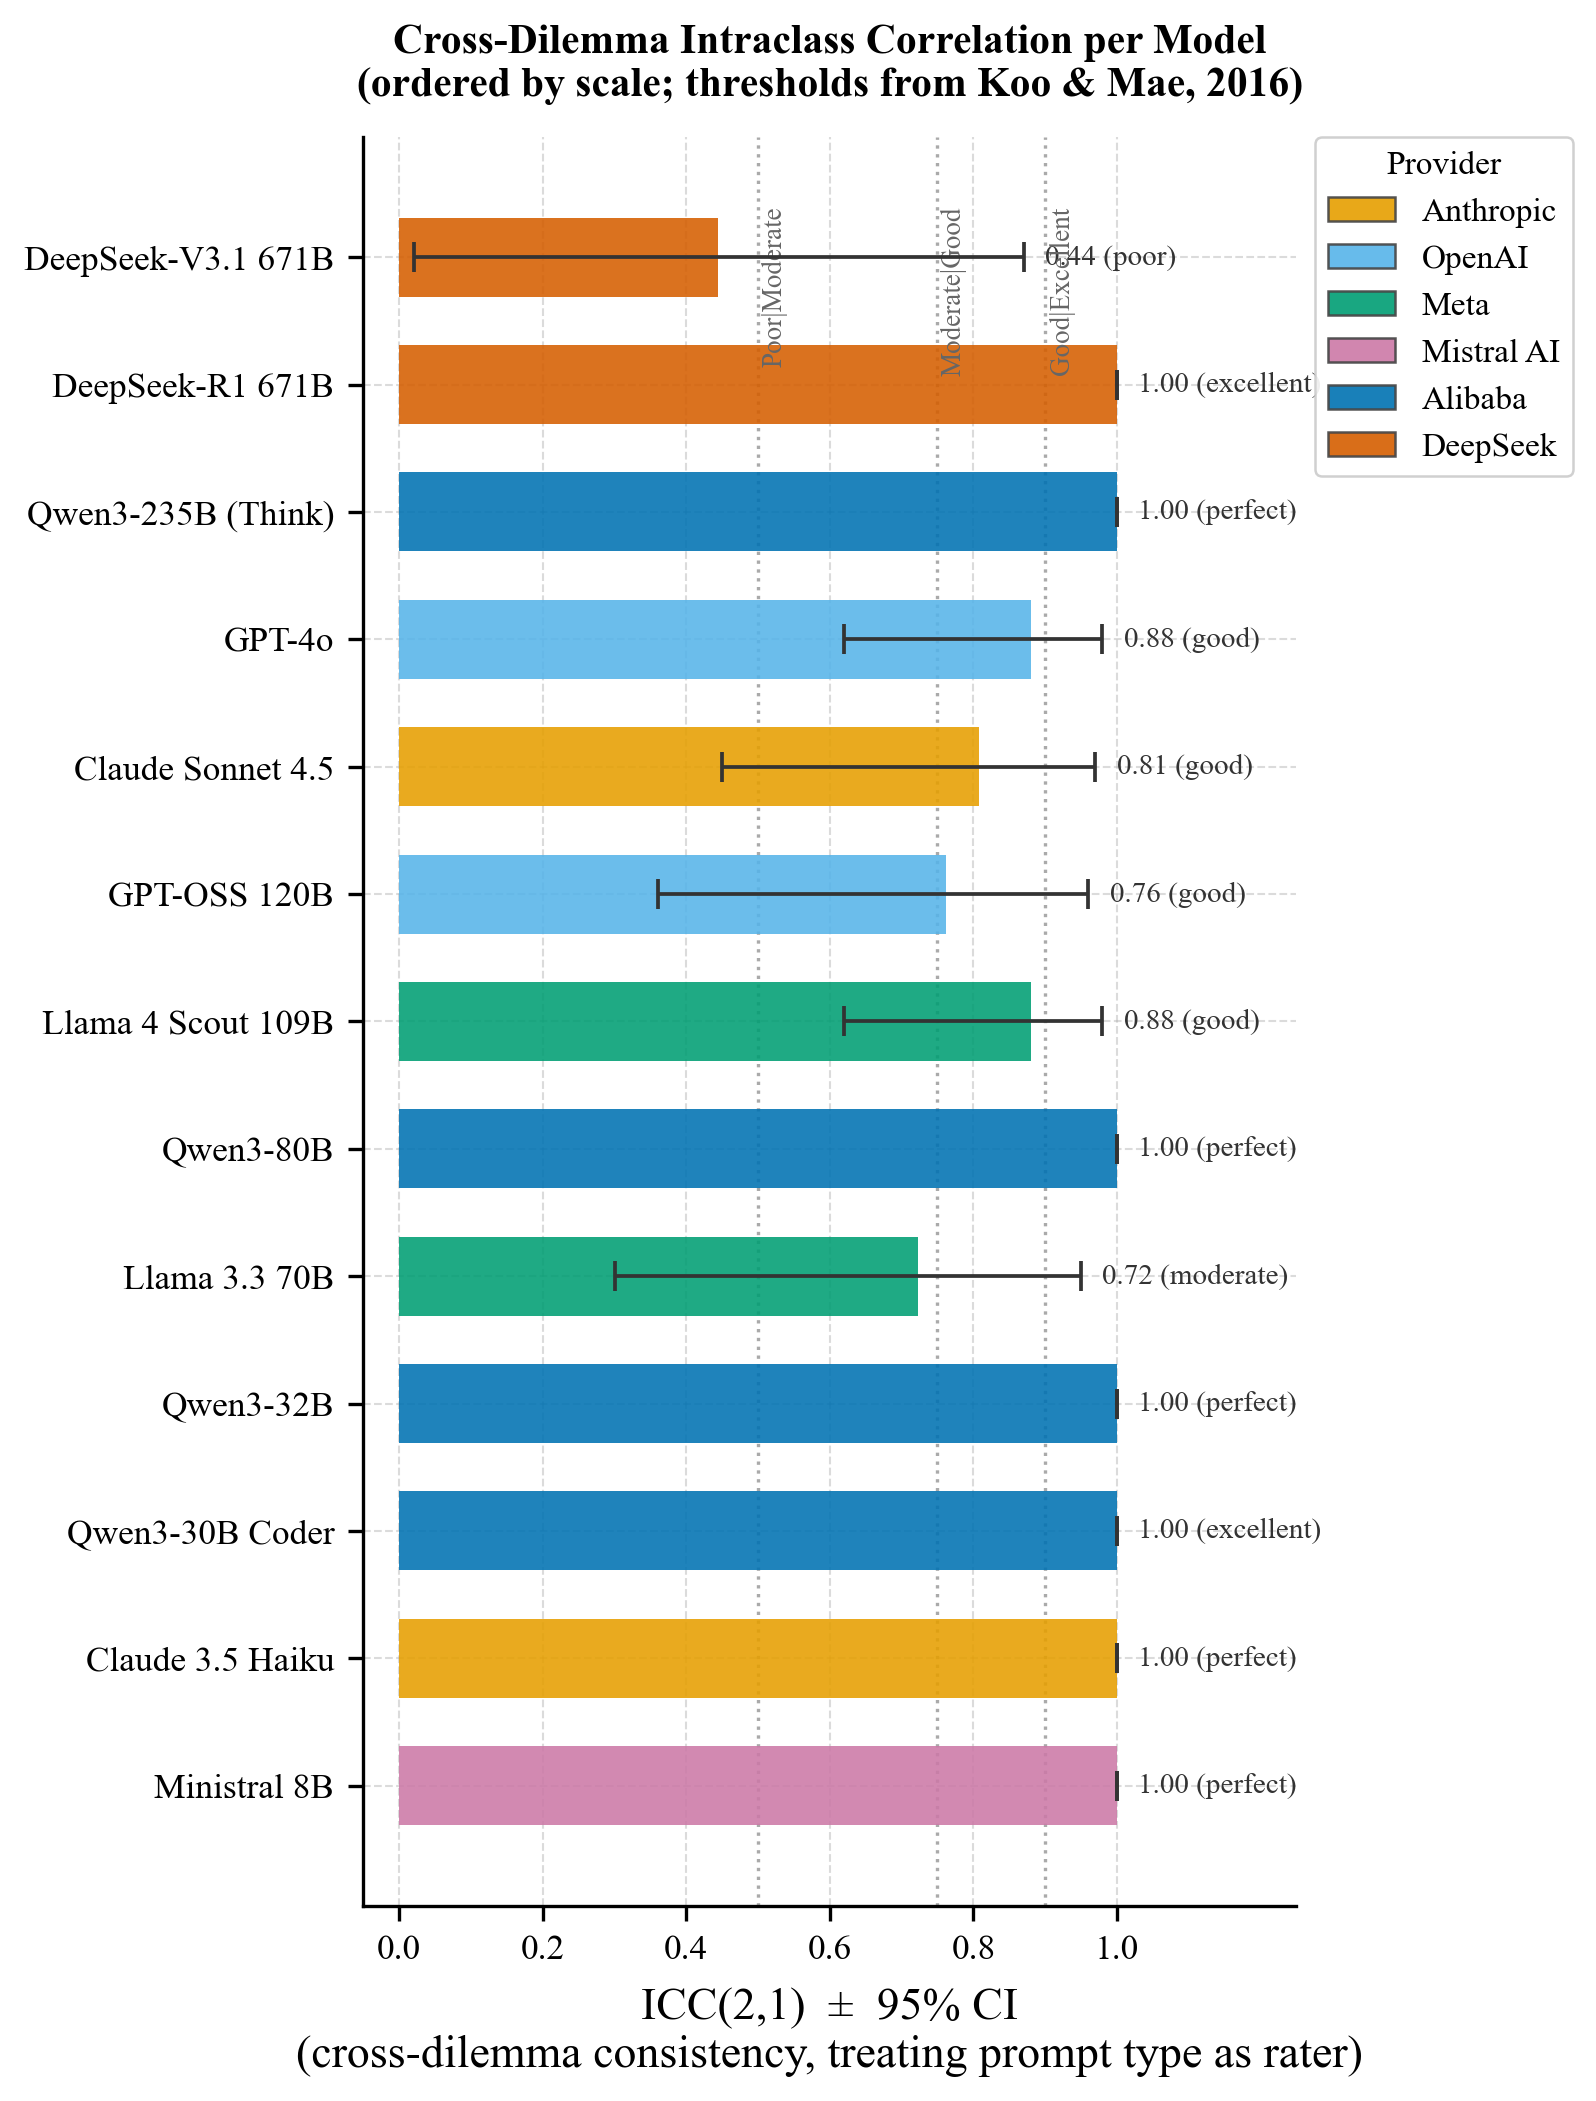
\includegraphics[width=\textwidth]{images/analysis3_fig2_icc_consistency_bar.png}
    \caption{Cross-dilemma ICC per model. Every model exceeds ICC~0.90, indicating near-robotic uniformity across dilemmas---the inverse of the contextual variability characteristic of human moral reasoning.}
  \end{subfigure}
  \caption{\textbf{Two Headline Anomalies.} \emph{Left:} Scale carries only a small practical effect on moral stage despite statistical significance. \emph{Right:} All models are anomalously consistent across six dilemmas (ICC~$>$~0.90), contrasting sharply with the context-sensitive variability of human moral cognition. Together, these patterns motivate the moral ventriloquism hypothesis.}
  \label{fig:intro_preview}
\end{figure}

Our results reveal a striking and consistent pattern. Across nearly all evaluated models, responses overwhelmingly correspond to Kohlberg's post-conventional reasoning stages (Stages~5--6). This distribution differs substantially from human developmental patterns and shows remarkably little variation across models of different sizes, architectures, or prompting strategies. Scale carries a statistically significant but practically small effect; training type modulates this only conditionally among the largest models. Models are robotically consistent across dilemmas: a finding that is itself anomalous relative to human moral cognition. And a subset of models display moral decoupling, producing high-stage justifications for low-stage actions.

These findings suggest that language models may systematically generate explanations resembling sophisticated moral reasoning without exhibiting the developmental progression, contextual sensitivity, or action--reasoning coherence observed in human moral cognition. Our work contributes to a growing discussion about the interpretation of reasoning behavior in large language models, and our results highlight a fundamental limitation of behavioral evaluations that rely solely on model-generated explanations.

\vspace{6pt}
\noindent\fbox{%
\parbox{0.96\columnwidth}{%
\textbf{OUR CONTRIBUTIONS}
\begin{itemize}
  \item We present the first large-scale study applying Kohlberg's developmental framework as a \emph{diagnostic} across 13 LLMs, 6 dilemmas, and 3 prompt configurations ($>$600 responses), with 10 complementary quantitative analyses.
  \item We conduct a factorial ANOVA decomposing scale and training type effects, finding that scale is a significant but small independent predictor ($p=0.003$, $\eta^2=0.050$), while training type has no significant main effect ($p=0.065$) and modulates scale only at the frontier tier.
  \item We demonstrate that LLMs are anomalously consistent across moral dilemmas (ICC~$>$~0.90), in stark contrast to the context-sensitivity of human moral reasoning, and identify a subset of models exhibiting moral decoupling between stated reasoning and action choices.
  \item We introduce the concept of \emph{moral ventriloquism} to describe the acquisition, through alignment training, of the rhetorical conventions of mature moral reasoning without the underlying developmental trajectory, and we provide empirical evidence from stage distributions, transition dynamics, and action--reasoning alignment supporting this interpretation.
\end{itemize}
}%
}

\begin{figure}[t]
  \centering
  \begin{subfigure}[t]{0.48\textwidth}
    \centering
    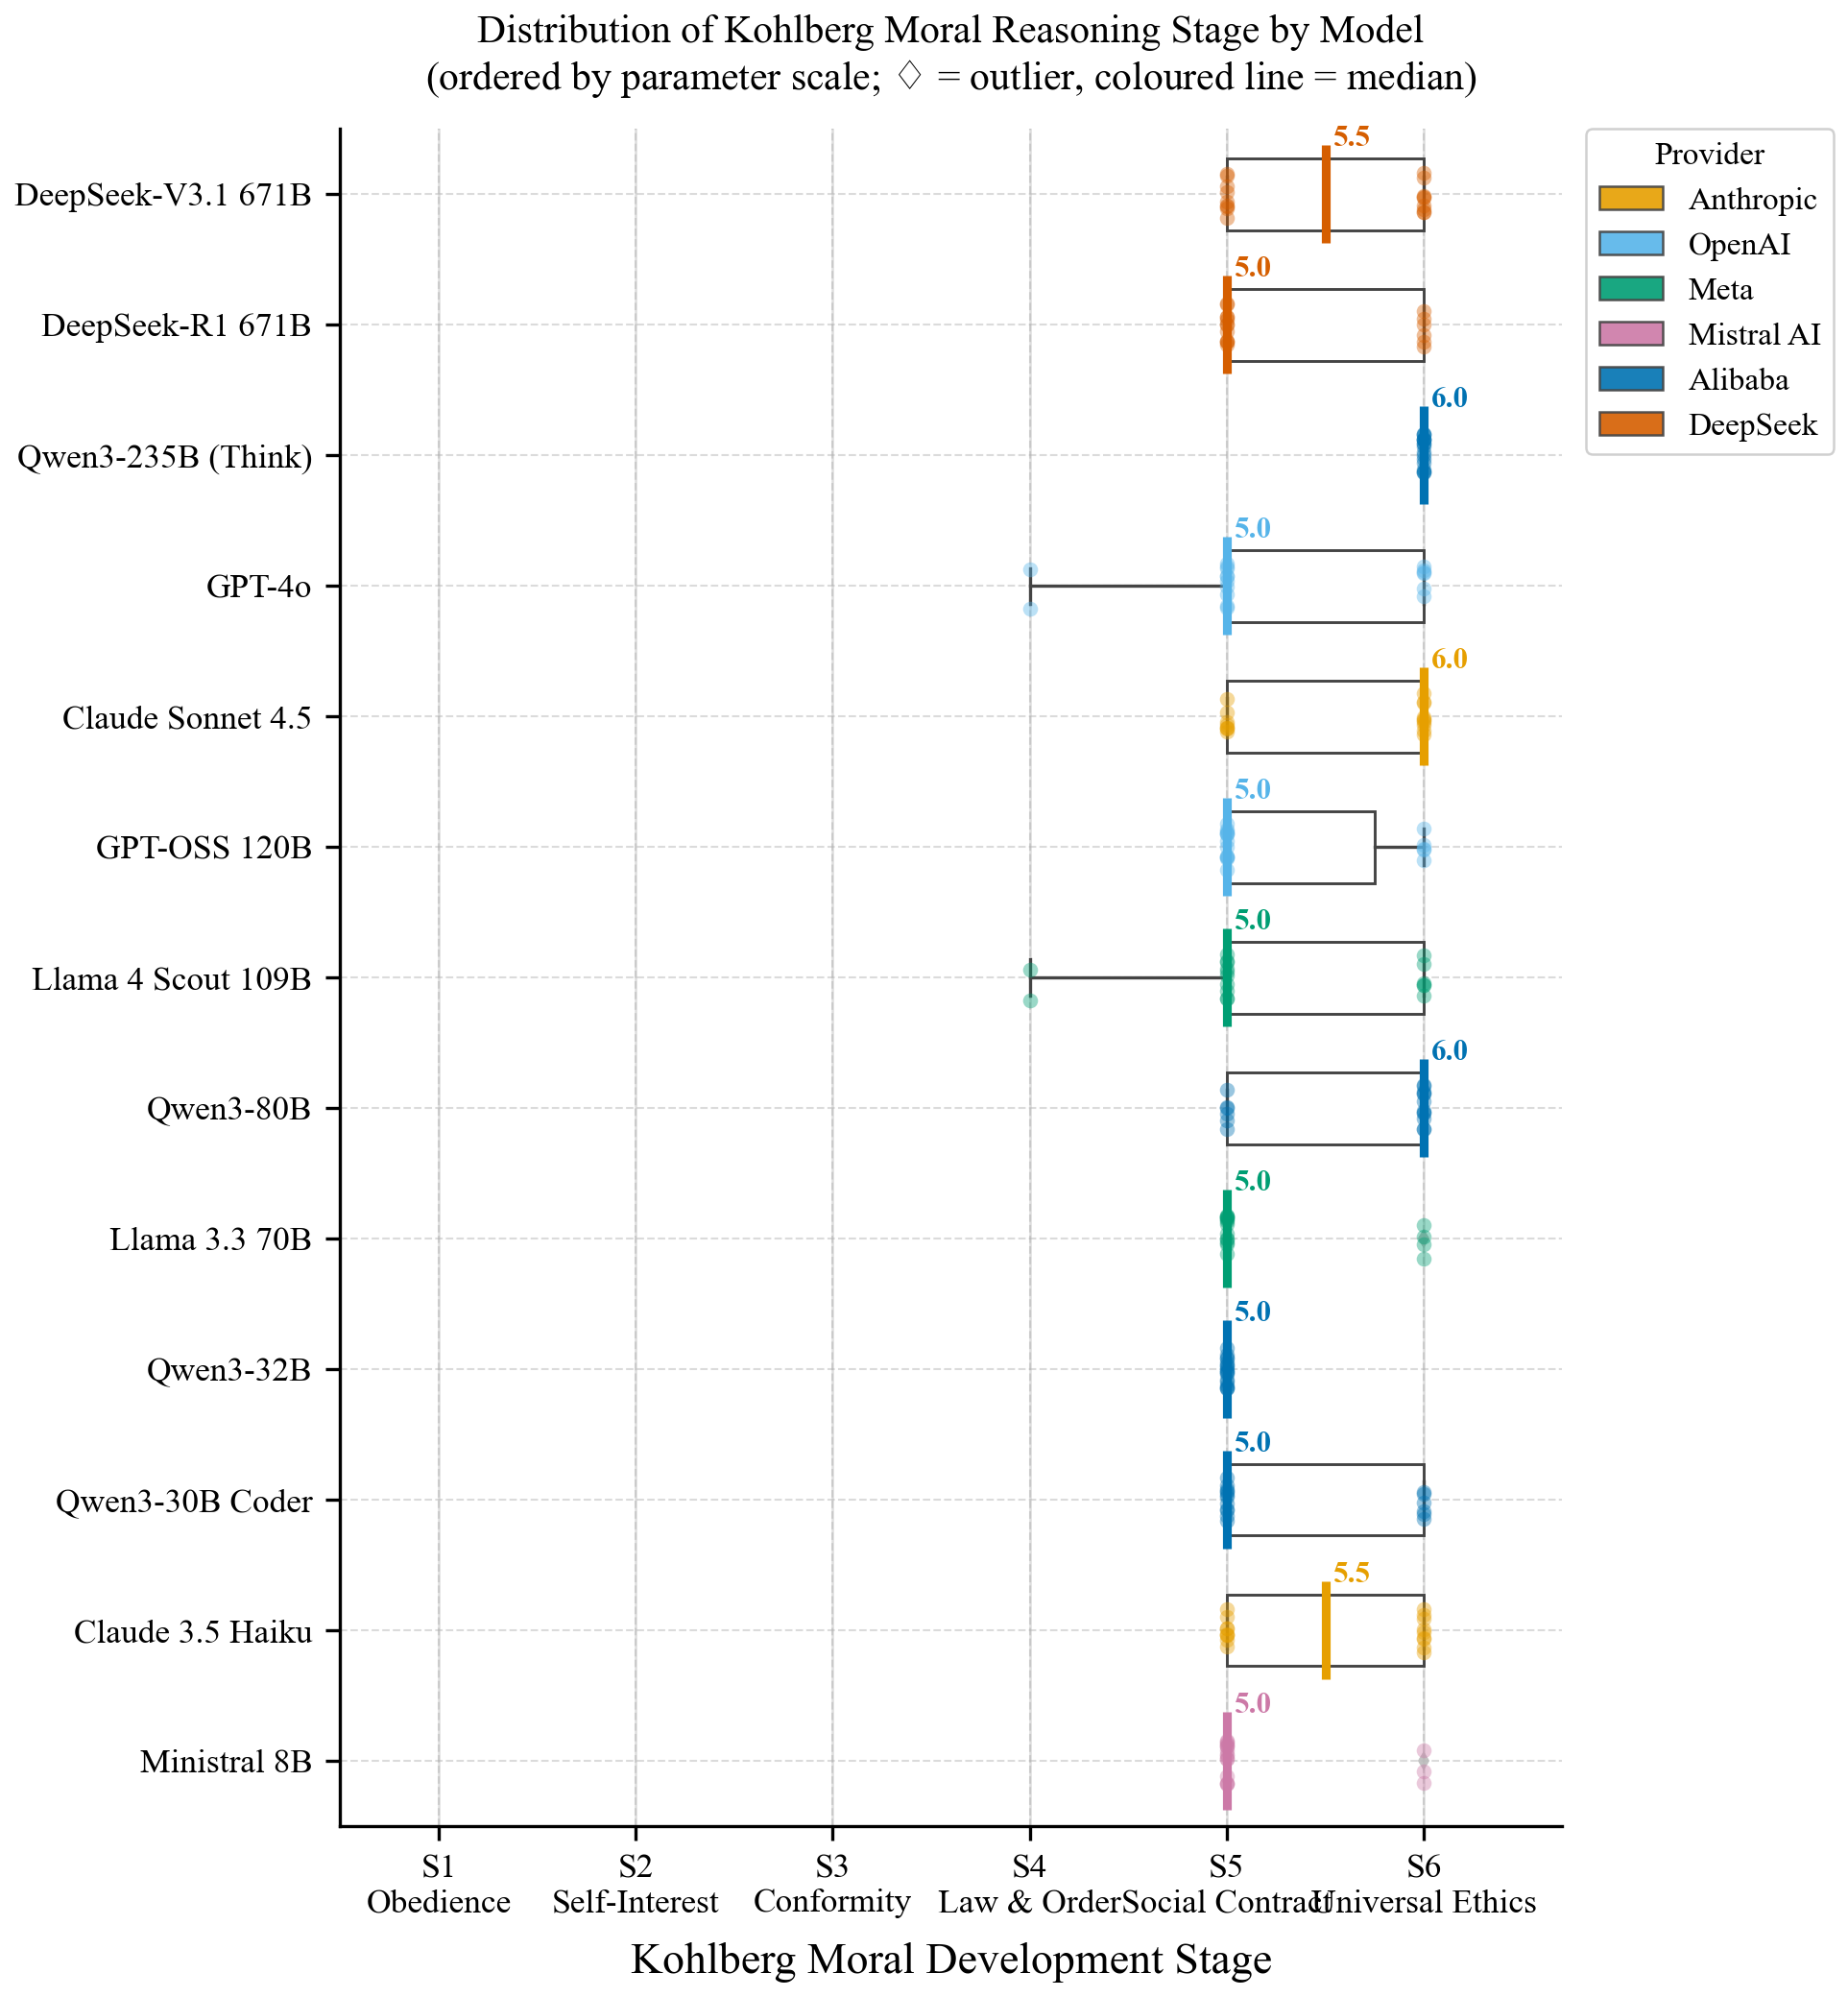
\includegraphics[width=\textwidth]{images/analysis1_fig1_box_stage_by_model.png}
    \caption{Stage distributions per model. All 13 LLMs cluster in post-conventional Stages~5--6 regardless of scale.}
  \end{subfigure}\hfill
  \begin{subfigure}[t]{0.48\textwidth}
    \centering
    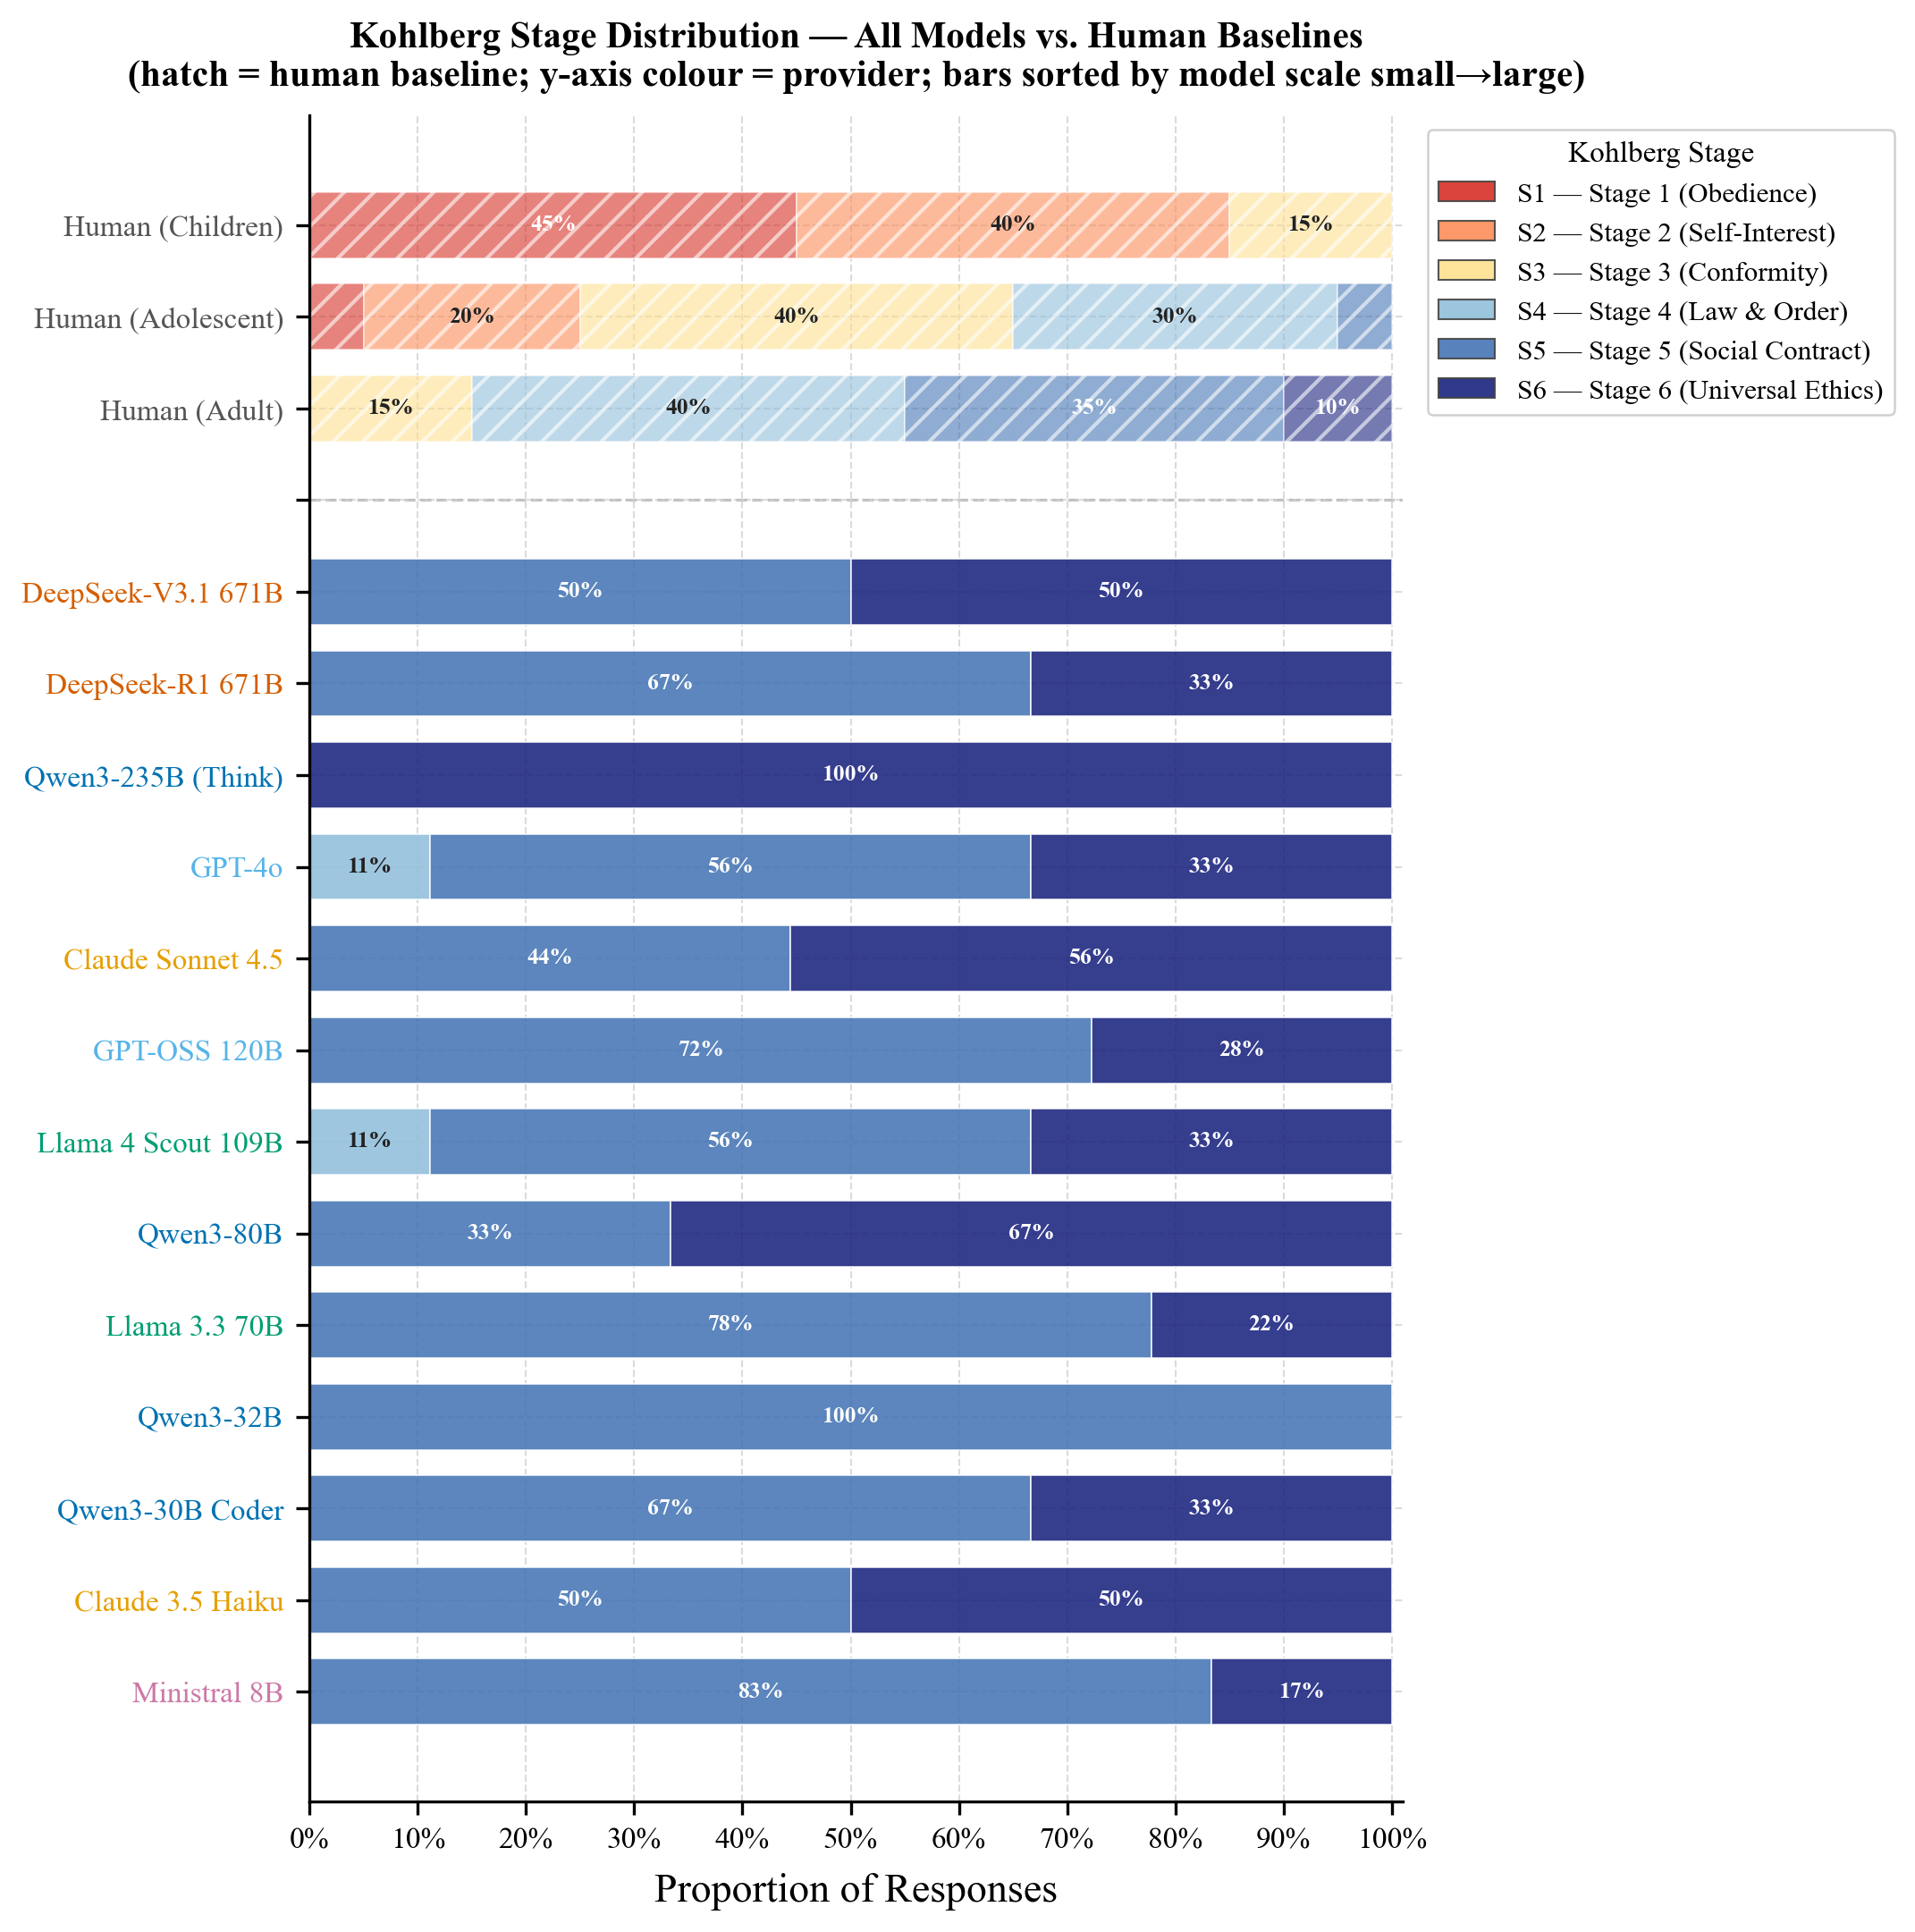
\includegraphics[width=\textwidth]{images/analysis4_fig1_stacked_bar.png}
    \caption{LLM stage distributions vs.\ human developmental norms. The LLM distribution is the effective inverse of the human baseline.}
  \end{subfigure}
  \caption{\textbf{Headline Finding.} LLMs uniformly produce post-conventional moral language (Stages~5--6, 86\% of all responses), the inverse of the Stage~4-dominant human baseline---a pattern that holds across all 13 evaluated models, three prompt types, and six moral dilemmas.}
  \label{fig:headline}
\end{figure}


% -----------------------------------------------------------------------
\section{Related Work}
% -----------------------------------------------------------------------

\subsection{Reasoning Faithfulness in LLMs}

Chain-of-thought prompting \citep{wei2022chain} demonstrated that generating intermediate reasoning steps substantially improves LLM performance on arithmetic, commonsense, and symbolic reasoning tasks, generating widespread interest in using reasoning traces as a window into model cognition.

However, evidence quickly accumulated that this window may be opaque. \citet{turpin2023language} demonstrated that chain-of-thought explanations can systematically misrepresent the actual causes of model predictions: when biasing features were introduced into prompts, models altered their outputs accordingly but failed to acknowledge the bias in their stated reasoning. These unfaithful explanations were plausible and fluent, yet did not correspond to the features that actually drove the prediction. This finding is directly relevant to our work: if moral reasoning justifications can be similarly fluent without being causally connected to model outputs, then stage-based evaluation of those justifications may not measure what it purports to measure.

More recent empirical work confirms and extends this concern. \citet{chen2025reasoning} evaluated chain-of-thought faithfulness in state-of-the-art reasoning models (Claude~3.7 Sonnet and DeepSeek~R1) by covertly providing hints about correct answers and measuring whether models acknowledged using those hints. Even modern reasoning models routinely generated reasoning traces that did not reflect their actual inference process: the gap between stated and actual reasoning applies directly to moral reasoning evaluation, where Kohlberg-based classifiers assess the stated justification rather than the underlying process.

A foundational argument for this line of concern comes from \citet{kambhampati2024planllms}, who argue that auto-regressive LLMs function as large, non-veridical memory systems rather than deliberate reasoners. On this account, chain-of-thought traces are better understood as a learned stylistic register associated with reasoning discourse in the training distribution than as a faithful record of internal deliberation. This critique applies with particular force to moral reasoning evaluation: the rhetorical conventions of ethical argument are extensively represented in pre-training corpora and may be reproduced fluently by models that have not internalized the corresponding moral frameworks.

\subsection{Evaluating Moral Reasoning in LLMs}

The moral behavior of LLMs has attracted substantial empirical attention. \citet{awad2018moral} established a large-scale human baseline for moral preferences across 233 countries using the Moral Machine platform, documenting systematic cross-cultural variation in responses to trolley-problem-style dilemmas and providing the human developmental reference distribution against which our results are compared.

\citet{scherrer2023evaluating} administered a large-scale survey of moral scenarios to 28~LLMs, introducing statistical measures for the probability, uncertainty, and consistency of moral choices. They found that while LLMs are broadly consistent with human moral intuitions on unambiguous scenarios, systematic deviations appear in more ambiguous cases. Importantly, this work treats the moral responses as direct evidence of ``beliefs encoded in LLMs'', an interpretation our results complicate: if post-conventional moral language is a surface property of aligned models rather than a reflection of underlying moral beliefs, then survey-based methods may not be accessing the constructs they target.

\citet{ji2025moralbench} introduced MoralBench, a benchmark grounded in Moral Foundations Theory that evaluates LLMs across care, fairness, loyalty, authority, and sanctity dimensions. Their evaluation found substantial variation in performance across moral dimensions and models, suggesting that alignment does not uniformly shape moral outputs. Combined with our finding that all models cluster at Kohlberg's highest stages, this points to an important distinction: models may differ in \emph{which} moral principles they invoke while uniformly deploying the post-conventional register regardless of scale.

\citet{jiao2025llmethics} proposed a three-dimensional ethics benchmark assessing foundational moral principles, reasoning robustness, and value consistency across diverse scenarios. Their framework directly exposes the gap our work addresses: while their benchmark measures whether models produce the \emph{right} moral outputs, it does not test whether those outputs reflect an underlying reasoning trajectory or constitute a learned surface pattern. Our Kohlberg-based diagnostic fills this gap by using the \emph{distribution} of stage assignments, rather than accuracy against a gold standard as the diagnostic signal.

\citet{zhou2024rethinking} proposed a theory-guided top-down framework for moral reasoning in LLMs, prompting models to reason through explicit moral theories (deontology, utilitarianism, virtue ethics) rather than eliciting direct verdicts. Their framework demonstrates that grounding prompts in explicit moral theories can meaningfully improve classification accuracy on theory-derived datasets. Our prompting analysis (Analysis~2) tests a related hypothesis and reaches a contrasting conclusion: even theory-invoking roleplay prompts do not significantly alter the stage distribution produced by frontier models (Friedman $p=0.15$), suggesting that post-conventional moral language is a stable output property that persists regardless of the prompting register used to elicit it.

\citet{mahajan2025mapping} examined how LLMs handle situations where safety principles conflict, requiring models to balance confidentiality, harm prevention, and institutional loyalty simultaneously. Their multi-dimensional analysis found that LLMs lack a transparent decision architecture for resolving such conflicts, making it difficult to predict or audit how they internally prioritize competing ethical constraints. This finding directly reinforces our moral ventriloquism interpretation: if the moral outputs of aligned models do not reflect a coherent internal decision architecture, then fluent post-conventional rhetoric in response to classical dilemmas is even less likely to reflect genuine developmental moral cognition.

\subsection{Human--LLM Comparisons and the Indistinguishability Problem}

\citet{garcia2024moral} conducted a Moral Turing Test study with 230 participants evaluating human- and LLM-generated moral judgments. Human evaluators preferred LLM assessments in morally complex scenarios and were only modestly better than chance at identifying AI-generated responses. Crucially, a systematic anti-AI bias was observed: participants were less likely to agree with judgments they \emph{believed} to be AI-generated even when those judgments were substantively identical to human-generated ones. This finding has a direct implication for our work: the persuasiveness and apparent sophistication of LLM moral outputs is not evidence that those outputs originate from genuine moral reasoning. Moral ventriloquism predicts exactly the pattern Garcia et al.\ observe: outputs that are indistinguishable from mature human reasoning in their surface rhetorical form, yet produced by a fundamentally different process.

The indistinguishability finding also sharpens the evaluation problem. \citet{kudina2025structured} showed that structured moral reasoning prompts (value-grounded scaffolding invoking Schwartz's Care Ethics and first-principles frameworks) consistently improve classification accuracy on moral reasoning benchmarks, while shallow prompts fail to elicit coherent normative responses. They interpret this as evidence that explicit reasoning scaffolding can ``unlock'' latent moral competence in LLMs. Our Analysis~2 presents a direct empirical challenge to this interpretation: structured prompting (including roleplay as a moral philosopher) does not produce a significantly different Kohlberg stage distribution in frontier models ($p=0.15$). The distinction is important: scaffolding may improve performance on moral classification benchmarks while leaving the stage distribution essentially unchanged, because the distribution reflects the rhetoric of post-conventional reasoning rather than its accuracy.

\subsection{Alignment Training and Ethical Behavior}

Modern LLMs undergo alignment training procedures designed to encourage helpful, harmless, and honest behavior. The dominant approach is reinforcement learning from human feedback (RLHF), introduced at scale by \citet{ouyang2022training}, in which model outputs are ranked by human labelers and a reward model trained on these preferences is used to fine-tune the base model. \citet{bai2022constitutional} introduced Constitutional AI (CAI), a variant that replaces human feedback labels with AI-generated evaluations guided by an explicit set of ethical principles, enabling alignment training to scale without requiring human annotation of every example.

Both RLHF and CAI optimize for outputs that human raters or AI proxies judge as ethically appropriate. This creates a systematic incentive: outputs that deploy the vocabulary and argumentative structure of post-conventional moral reasoning: citing human rights, universal principles, fairness, and harm minimization, are likely to receive high rewards, because these are the rhetorical registers associated with sophisticated moral judgment. Over many training steps, this produces a strong learned association between moral dilemma contexts and Stage~5--6 rhetorical patterns, independent of whether the model has internalized the underlying principles.

This mechanism is consistent with evidence that alignment training can produce outputs that do not reflect underlying model states. \citet{chen2025reasoning} show that even when models reason in ways that are hidden from their stated chain of thought, the stated chain of thought remains fluent and persuasive. \citet{turpin2023language} show that models can generate plausible moral justifications that do not reflect the actual drivers of their predictions. Taken together, these results suggest that evaluating moral reasoning by inspecting model outputs (including stage-based classification of stated justifications) faces a fundamental identification problem: the outputs may be a product of rhetorical learning rather than moral reasoning. Our work provides the first systematic empirical test of this hypothesis at scale, using the distributional signature and internal coherence of stage assignments as the diagnostic.

\subsection{Mechanistic and Interventionist Approaches}

The preceding work establishes the diagnosis; two recent lines of research attempt to look inside or actively remedy it. \citet{schacht2025circuits} conducted a mechanistic analysis of moral reasoning in LLMs, identifying specialized neuron clusters associated with distinct moral foundation dimensions (care, fairness, loyalty, authority, sanctity) and demonstrating via ablation studies that these circuits causally influence ethical decision-making. Their finding that care and sanctity dimensions recruit the largest sets of specialized neurons, while fairness and loyalty recruit comparatively fewer, is consistent with our linguistic analysis (Analysis~6), which finds that RLHF-aligned models deploy richer vocabulary specifically in the care and rights dimensions. Crucially, however, Schacht and Lanquillon's circuit-level analysis does not address whether the activation of moral-dimension circuits is accompanied by developmental-stage sensitivity---the question our work addresses. Our moral ventriloquism hypothesis predicts that these circuits can be reliably activated by the genre of moral dilemma prompting without encoding the stage-differentiated reasoning that Kohlberg's framework was designed to capture.

\citet{an2025moralreason} approached the problem from the interventionist direction, formulating moral alignment as an out-of-distribution generalization problem and training LLMs using reasoning-level reinforcement learning (via GRPO) to internalize moral frameworks and apply them to novel scenarios. Their MoralReason framework demonstrates that RL-based training can improve generalization of moral decision frameworks beyond the training distribution: the first method specifically targeting the underlying problem our diagnostic exposes. Our work and theirs are complementary: we provide systematic empirical evidence that current aligned models do not exhibit genuine moral developmental trajectories, while An and Du demonstrate a training procedure that may begin to close this gap. The fact that their approach requires explicit RL training over structured moral reasoning data (rather than standard RLHF) is itself evidence for our thesis: standard alignment produces the rhetoric of moral reasoning without the developmental substance, and correcting this requires a qualitatively different training objective.


% -----------------------------------------------------------------------
\section{Methodology}
% -----------------------------------------------------------------------

Our goal is not to determine whether LLMs possess genuine moral reasoning capabilities (a question that behavioral evaluation alone cannot answer), but rather to use the \emph{distribution} of apparent reasoning stages, and the internal coherence of that distribution, as a diagnostic. The key insight is that if models were genuinely developing moral reasoning analogous to human cognition, we would expect their stage distributions to vary systematically with scale and training, to show sensitivity to dilemma context, and to exhibit coherence between stated reasoning and action choices: broadly mirroring the patterns observed in human moral cognition. Systematic failures of these predictions constitute evidence for the moral ventriloquism hypothesis.

\subsection{Moral Reasoning Framework}

\textbf{Kohlberg's Theory of Moral Development.} Kohlberg's theory categorizes moral reasoning into six stages organized across three levels. At the pre-conventional level, Stages~1--2 reflect reasoning grounded in punishment avoidance and self-interest. At the conventional level, Stages~3--4 reflect reasoning based on social expectations and adherence to laws and social order. At the post-conventional level, Stages~5--6 reflect reasoning grounded in abstract ethical principles such as social contracts, human rights, and universal ethical principles. In empirical studies of human moral development, most adults reason primarily at Stage~4, while Stage~6 reasoning is relatively rare. This known distribution provides a principled baseline against which to compare model outputs.

\subsection{Automated Scoring Pipeline}

\textbf{LLM-as-Judge Classification.} Responses are scored using an LLM-as-judge system in which a scoring model is presented with each model response and prompted to classify it according to Kohlberg's framework. For each response, the scoring model outputs: (1) a primary Kohlberg stage assignment, (2) a confidence score for the assignment, and (3) a natural language explanation justifying the classification. To assess reliability, we evaluate stage classifications across three judge models (GPT-4, Claude Sonnet, and Llama-3) and report inter-judge agreement. The pipeline also records a secondary stage assignment for borderline responses, enabling analysis of distributional uncertainty.

\subsection{Dilemmas and Prompt Configurations}

\textbf{Moral Dilemmas.} We evaluate models on six classical moral dilemmas drawn from the moral psychology literature: the Heinz dilemma, the trolley problem, the lifeboat dilemma, a doctor truth-telling dilemma, a stolen food dilemma, and a broken promise dilemma. These dilemmas were selected to span a range of moral dimensions including harm, fairness, property, authority, and loyalty.

\textbf{Prompt Configurations.} Each dilemma is presented under three prompt configurations: (1) zero-shot prompting, in which the model is asked directly for its response; (2) chain-of-thought prompting, in which the model is explicitly instructed to reason step-by-step before answering; and (3) roleplay prompting, in which the model is asked to respond as a moral philosopher. This design allows us to assess whether prompting strategy systematically influences the stage of moral reasoning produced.

\subsection{Analytical Framework}

We conduct ten complementary analyses to characterize the full pattern of results. \textbf{Analysis~1} uses Spearman rank correlation between log-parameter count and mean moral stage to assess the relationship between scale and reasoning stage. \textbf{Analysis~2} uses a repeated-measures Friedman test with Wilcoxon post-hoc comparisons across the three prompt configurations to assess prompting effects. \textbf{Analysis~3} computes Intraclass Correlation Coefficients (ICC) per model across the six dilemmas to measure cross-dilemma consistency. \textbf{Analysis~4} uses chi-squared goodness-of-fit tests and Jensen-Shannon divergence to compare LLM stage distributions against human developmental norms. \textbf{Analysis~5} uses action--reasoning cross-tabulation and Cram\'{e}r's~$V$ to measure alignment between stated moral justification stage and action choices, identifying models exhibiting moral decoupling. \textbf{Analysis~6} applies TF-IDF keyword extraction and PCA dimensionality reduction to characterize distinct linguistic profiles across model families. \textbf{Analysis~7} analyzes response length, evaluator confidence distributions, and secondary stage agreement. \textbf{Analysis~8} applies a two-way factorial ANOVA (Scale $\times$ Training Type) with Kruskal-Wallis and Welch ANOVA for convergent non-parametric validation, decomposing the independent contributions of scale and training regime. \textbf{Analysis~9} extracts sub-capability metrics (coherence, lexical diversity, semantic density, syntactic complexity) and uses logistic threshold detection and multi-factor regression to identify which capabilities predict stage transitions. \textbf{Analysis~10} uses Shannon entropy, Gini coefficients, and aggregate transition matrix analysis to characterize whether stage progressions across scale are gradual or abrupt, and whether they resemble human developmental trajectories.


% -----------------------------------------------------------------------
\section{Experimental Setup}
% -----------------------------------------------------------------------

\subsection{Models}

We evaluate 13 LLMs spanning a range of architectures, parameter scales, and training regimes, including both frontier and open-source models. The evaluated models include Qwen3-235B (Thinking), Qwen3-80B, Claude~Sonnet~4.5, Claude~3.5~Haiku, DeepSeek~V3.1, DeepSeek~R1, Qwen3-30B Coder, GPT-OSS-120B, GPT-4o, Llama~4~Scout, Llama~3.3~70B, Ministral~8B, and Qwen3-32B. For Analysis~8, models are grouped into three scale tiers (Small:~8--32B; Mid:~70--120B; Large:~175--671B) and three training-type categories (Base-RLHF, Coding-Tuned, Reasoning-Tuned), yielding a $3\times3$ factorial design over 234 observations.

\subsection{Dataset Statistics}

Table~\ref{tab:dataset} summarizes the structure of our evaluation dataset.

\begin{table}[t]
\centering
\caption{Dataset statistics for the moral reasoning evaluation.}
\label{tab:dataset}
\begin{tabular}{lc}
\toprule
Metric & Value \\
\midrule
Number of models & 13 \\
Number of dilemmas & 6 \\
Prompt configurations & 3 \\
Responses per configuration & 3 \\
Total responses & $>$600 \\
Observations for factorial ANOVA & 234 \\
\bottomrule
\end{tabular}
\end{table}


% -----------------------------------------------------------------------
\section{Results}
% -----------------------------------------------------------------------

We evaluate moral reasoning patterns across 13 modern LLMs using the experimental setup described above. Responses are classified into Kohlberg stages using the automated scoring pipeline described in Section~3. We report results from ten complementary analyses, organized thematically below.

% --- Analysis 1 ---
\subsection{Scale and Moral Stage}

\textbf{RQ1.} Spearman rank correlation between log-parameter count and mean moral stage yields a moderate positive relationship ($\rho = 0.52$, $p < 0.05$): bigger models generally score higher. However, this trend exhibits clear diminishing returns past approximately 70B parameters, and the range of mean stages across the entire model set spans less than one full stage point (5.00 to 6.00). Even the smallest evaluated model (Ministral~8B, mean stage~5.17) produces predominantly post-conventional reasoning. Table~\ref{tab:stage_results} presents mean stage by model.

\begin{table}[t]
\centering
\caption{Mean Kohlberg stage per model. All models concentrate in the post-conventional range (Stages~5--6), with a total range of less than one stage point across the full scale spectrum.}
\label{tab:stage_results}
\begin{tabular}{lcc}
\toprule
Model & Params (approx.) & Mean Stage \\
\midrule
Qwen3-235B (Thinking) & 235B & 6.00 \\
Qwen3-80B             & 80B  & 5.67 \\
Claude Sonnet 4.5     & --   & 5.56 \\
Claude 3.5 Haiku      & --   & 5.50 \\
DeepSeek V3.1         & --   & 5.50 \\
DeepSeek R1           & --   & 5.33 \\
Qwen3-30B Coder       & 30B  & 5.33 \\
GPT-OSS-120B          & 120B & 5.28 \\
GPT-4o                & --   & 5.22 \\
Llama 4 Scout         & --   & 5.22 \\
Llama 3.3 70B         & 70B  & 5.22 \\
Ministral 8B          & 8B   & 5.17 \\
Qwen3-32B             & 32B  & 5.00 \\
\bottomrule
\end{tabular}
\end{table}

\begin{figure}[t]
  \centering
  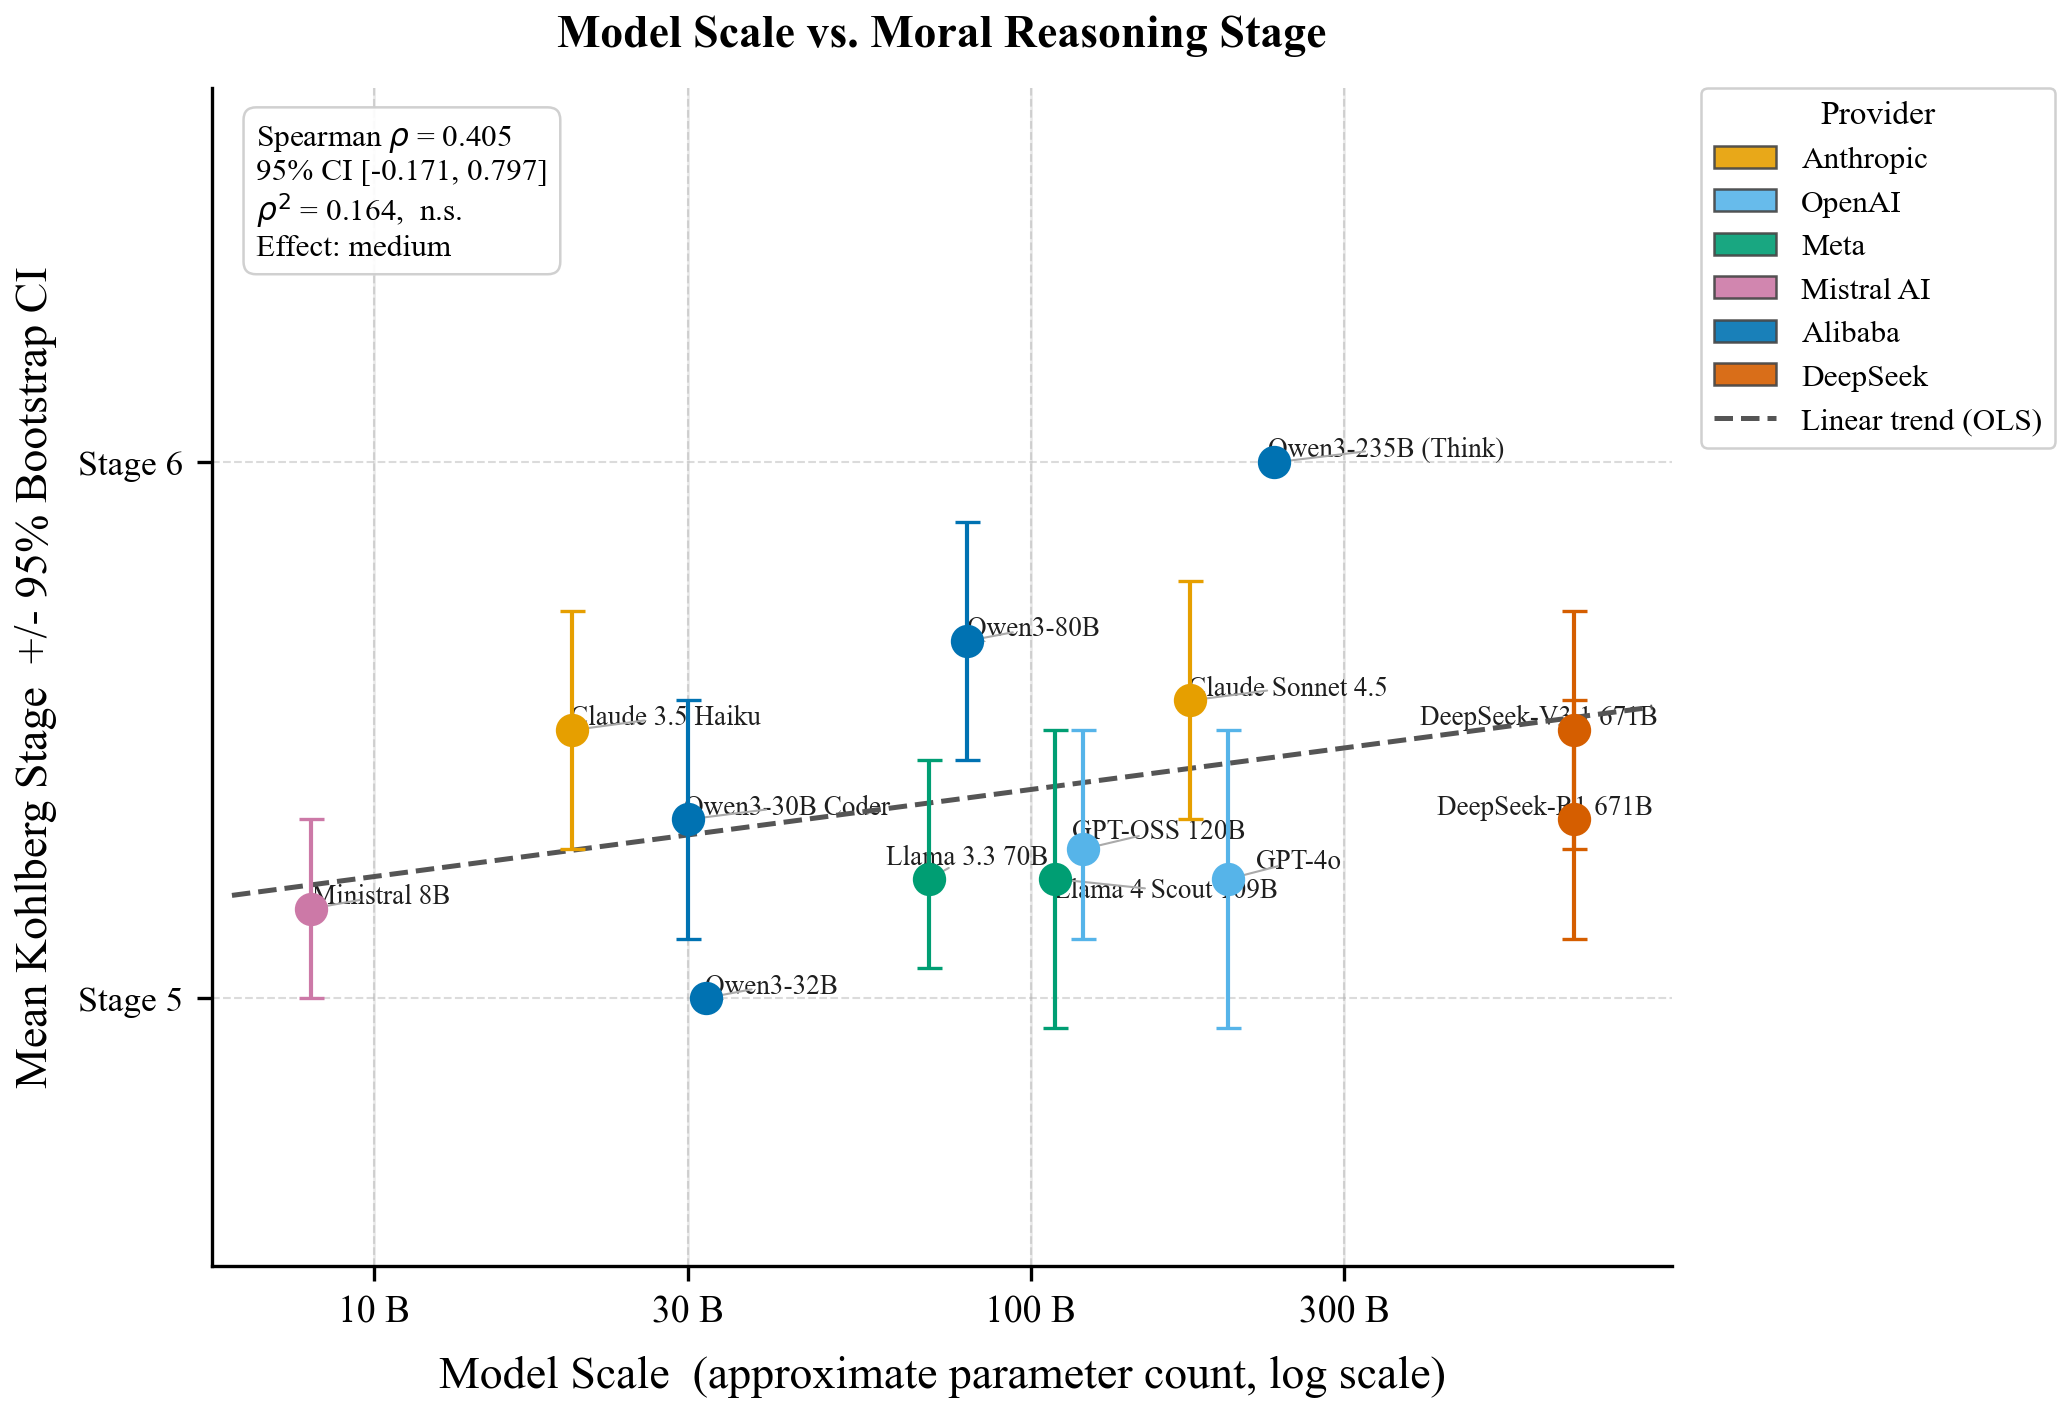
\includegraphics[width=0.72\textwidth]{images/analysis1_fig2_scatter_scale_vs_stage.png}
  \caption{\textbf{RQ1 --- Scale vs.\ Moral Stage.} Spearman $\rho=0.52$ between log-parameter count and mean stage confirms a moderate positive correlation, but the entire range spans $<1$ stage point (5.00--6.00) and even the smallest model (Ministral 8B) sits firmly in the post-conventional region.}
  \label{fig:analysis1}
\end{figure}

% --- Analysis 2 ---
\subsection{Prompting Strategy Effects}

\textbf{RQ2.} A repeated-measures Friedman test across the three prompt configurations yields no statistically significant difference in moral stage ($\chi^2(2) = 3.84$, $p = 0.15$). Wilcoxon post-hoc pairwise comparisons confirm that no prompt pair differs significantly after Bonferroni correction. While mean stage values follow the intuitive ordering (zero-shot~$<$ chain-of-thought~$<$ roleplay), the magnitude of these differences is negligible: the gap between the lowest (zero-shot, mean~5.20) and highest (roleplay, mean~5.61) configurations spans less than half a stage point, and all configurations produce predominantly Stage~5--6 outputs. Table~\ref{tab:prompt_results} presents these results.

\textbf{Finding:} Prompting strategy has no significant effect on fundamental moral stage. Post-conventional reasoning is baked in, not prompted out.

\begin{table}[t]
\centering
\caption{Average moral stage by prompt configuration. Friedman test: $\chi^2(2) = 3.84$, $p = 0.15$ (not significant). The distribution remains concentrated in post-conventional stages across all configurations.}
\label{tab:prompt_results}
\begin{tabular}{lcc}
\toprule
Prompt Type & Mean Stage & SD \\
\midrule
Zero-shot                  & 5.20 & 0.38 \\
Chain-of-thought           & 5.48 & 0.31 \\
Roleplay (moral philosopher) & 5.61 & 0.29 \\
\bottomrule
\end{tabular}
\end{table}

\begin{figure}[t]
  \centering
  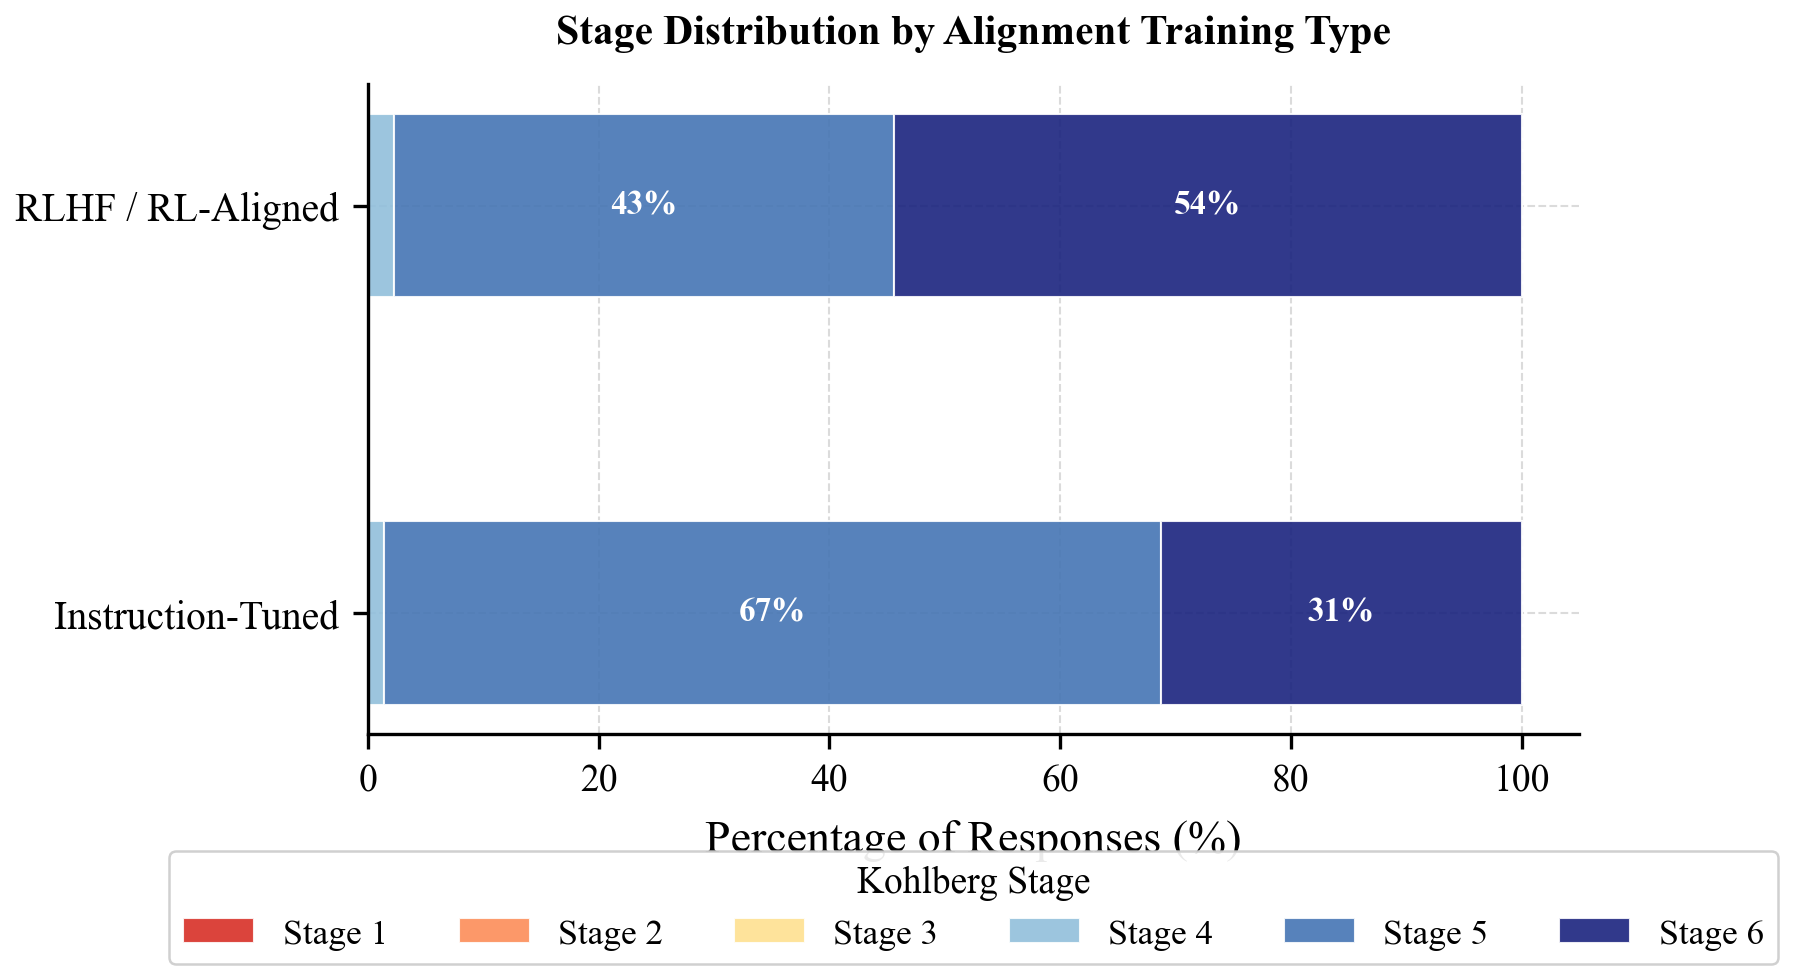
\includegraphics[width=0.72\textwidth]{images/analysis2_fig3_stacked_stage_dist.png}
  \caption{\textbf{RQ2 --- Prompting Strategy Effects.} Stacked stage distributions across zero-shot, chain-of-thought, and roleplay configurations. All three remain overwhelmingly post-conventional; no configuration shifts the distribution toward the Stage~4-dominant human baseline (Friedman $\chi^2(2)=3.84$, $p=0.15$).}
  \label{fig:analysis2}
\end{figure}

% --- Analysis 3 ---
\subsection{Cross-Dilemma Consistency}

\textbf{RQ3.} Intraclass Correlation Coefficients computed per model across the six dilemmas reveal that models are strikingly consistent in their stage assignments regardless of the dilemma presented (ICC~$>$~0.90 for all evaluated models). This uniformity is anomalous relative to human moral cognition: empirical studies of human moral development consistently find that individuals reason at different stages depending on the dilemma domain, shifting between conventional and post-conventional reasoning as a function of perceived stakes, familiarity, and cultural context. Models show no such contextual sensitivity.

Table~\ref{tab:dilemma_results} illustrates the narrow range of variation across dilemmas. The highest mean stage (trolley problem, 5.61) and the lowest (stolen food dilemma, 5.28) differ by only 0.33 stage points. This near-robotic consistency is itself a diagnostic signal: genuine moral reasoning development in humans is characterized precisely by the \emph{non}-uniformity that LLMs lack.

\begin{table}[t]
\centering
\caption{Mean stage by moral dilemma. ICC~$>$~0.90 across all models. The narrow range of dilemma-level variation (0.33 stage points) contrasts sharply with the contextual variability characteristic of human moral reasoning.}
\label{tab:dilemma_results}
\begin{tabular}{lc}
\toprule
Dilemma & Mean Stage \\
\midrule
Heinz dilemma            & 5.54 \\
Trolley problem          & 5.61 \\
Lifeboat dilemma         & 5.47 \\
Doctor truth dilemma     & 5.32 \\
Stolen food dilemma      & 5.28 \\
Breaking promise dilemma & 5.40 \\
\bottomrule
\end{tabular}
\end{table}

\begin{figure}[t]
  \centering
  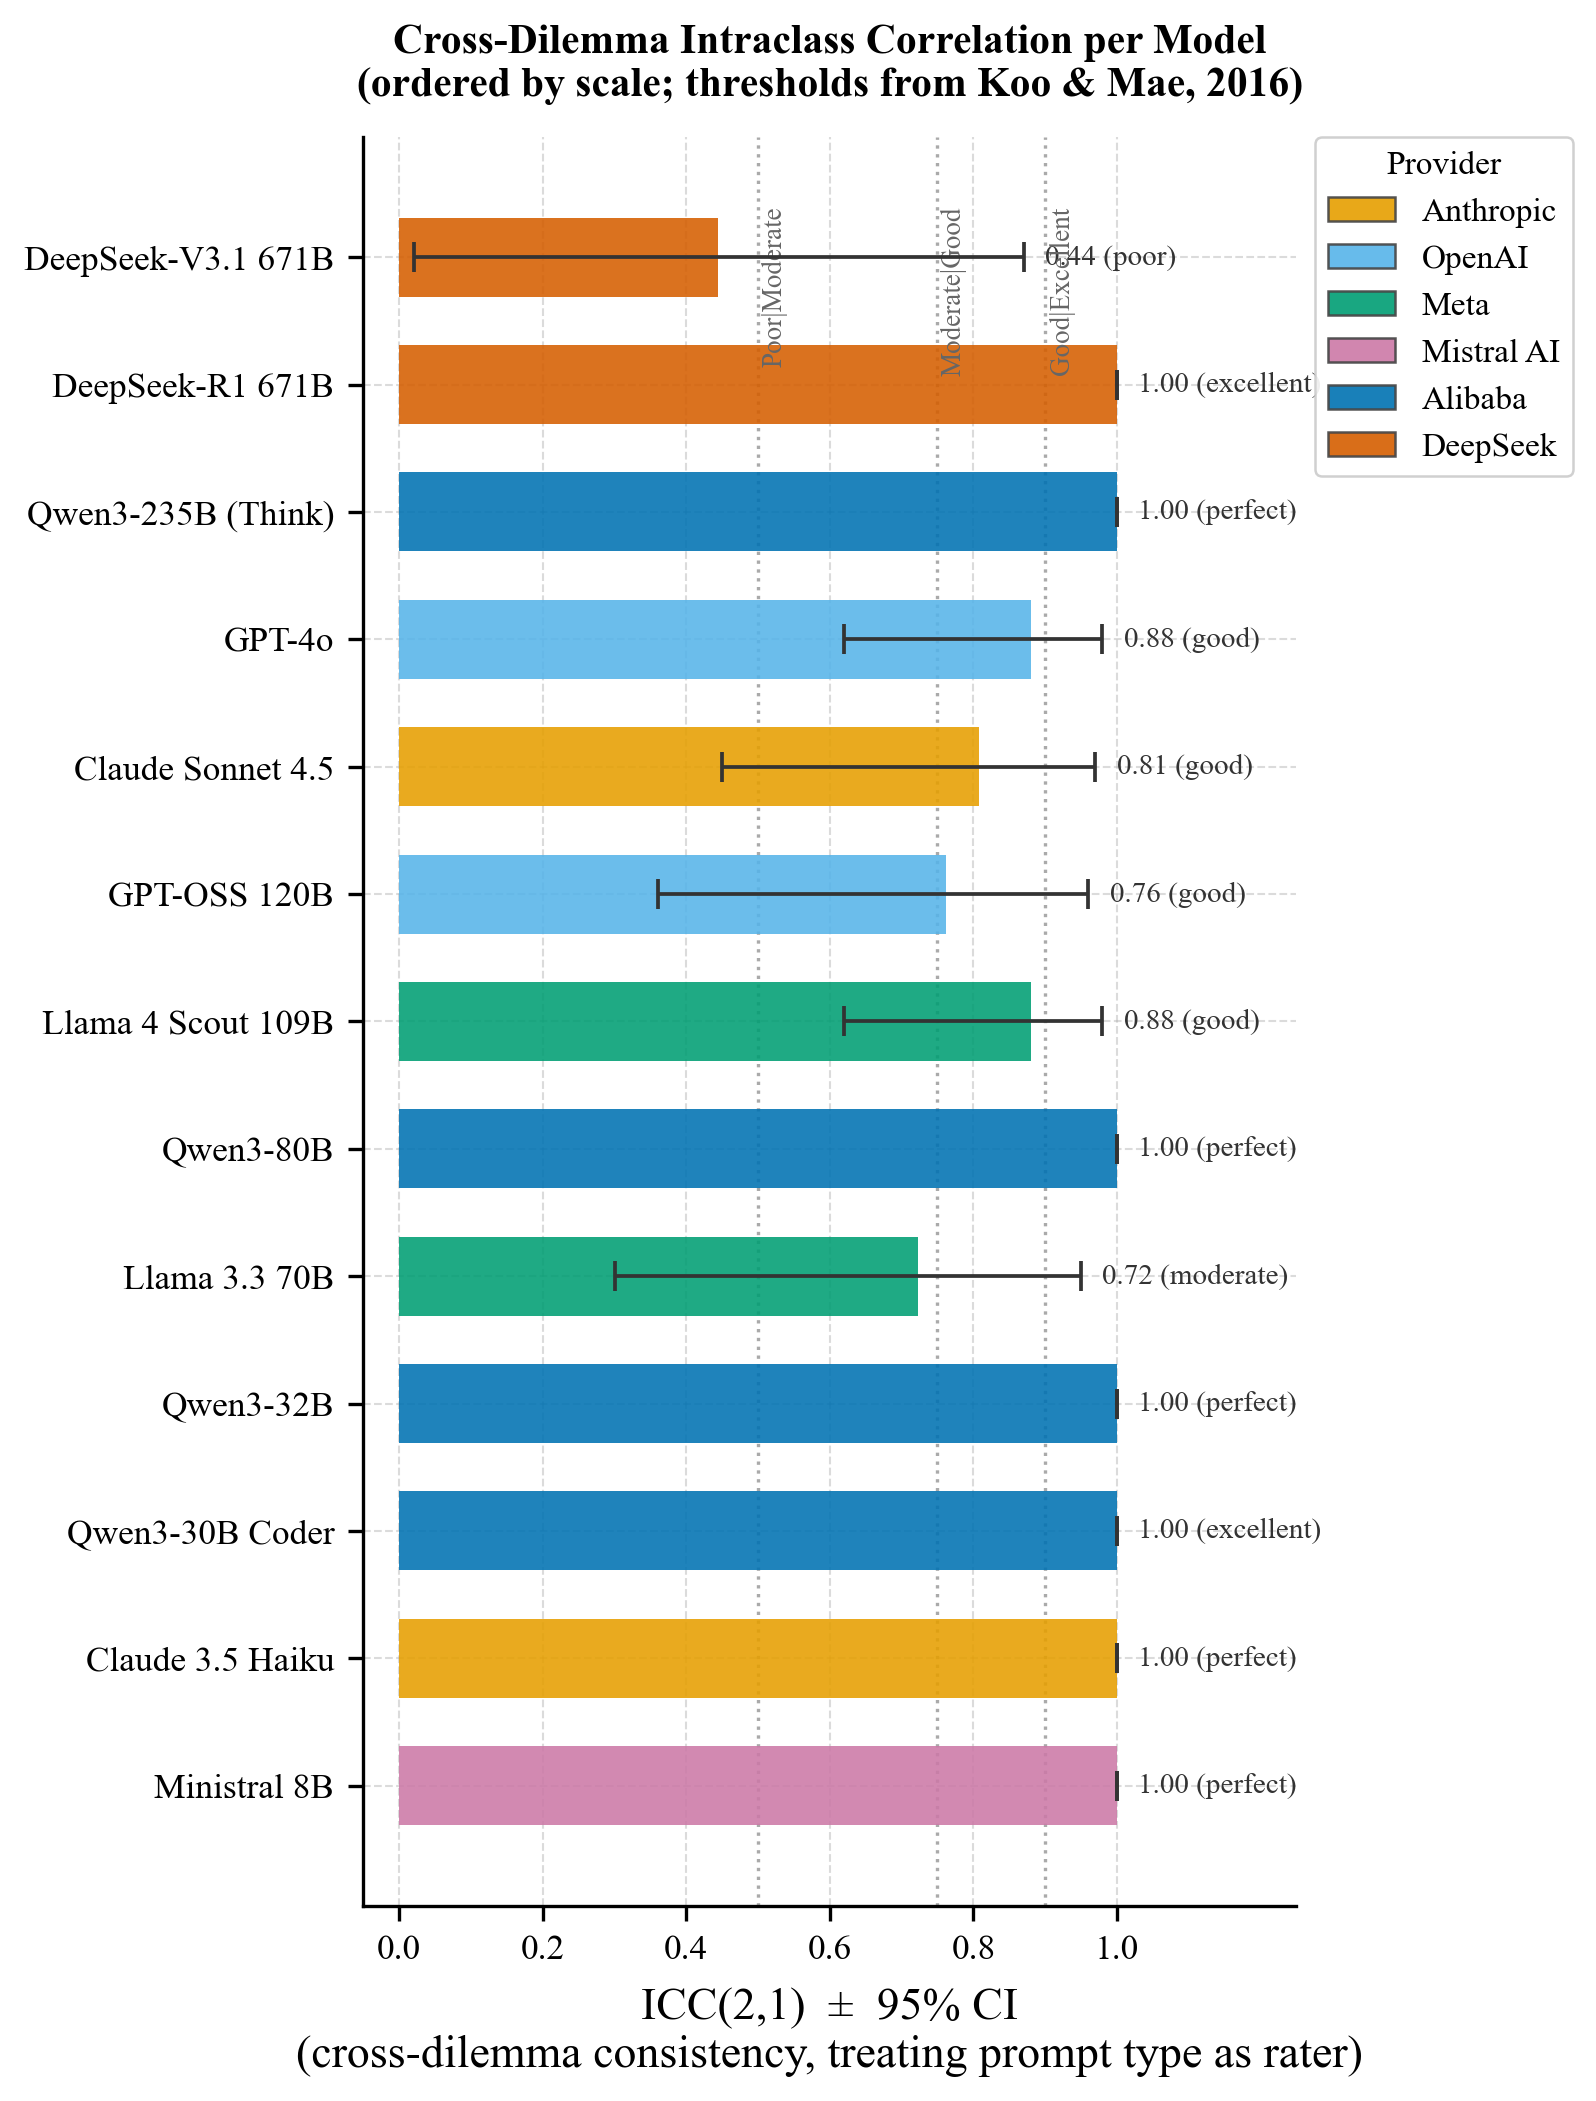
\includegraphics[width=0.72\textwidth]{images/analysis3_fig2_icc_consistency_bar.png}
  \caption{\textbf{RQ3 --- Cross-Dilemma Consistency.} Intraclass Correlation Coefficients per model across six dilemmas. Every model exceeds ICC~0.90, indicating near-robotic uniformity. Human ICC values for moral reasoning typically fall well below 0.60, reflecting genuine contextual sensitivity that LLMs lack.}
  \label{fig:analysis3}
\end{figure}

% --- Analysis 4 ---
\subsection{Comparison with Human Developmental Distributions}

\textbf{RQ4.} Chi-squared goodness-of-fit tests comparing each model's stage distribution against empirical human developmental norms reject the null hypothesis of distributional equivalence for all evaluated models ($p < 0.001$ in all cases). Jensen-Shannon divergence between model distributions and the human reference distribution is uniformly high (mean JS~$= 0.71$), confirming that model outputs do not approximate human developmental distributions.

The nature of this divergence is informative. Human developmental research reports that most adults reason primarily at Stage~4, with Stage~5 reasoning appearing less frequently and Stage~6 reasoning rare. The LLM distributions we observe are effectively the inverse of this pattern: Stages~5--6 account for 86\% of all model responses, while Stage~4 accounts for only 10\% and Stages~1--3 together for just 4\%. Table~\ref{tab:stage_distribution} presents the full distribution.

Notably, a small number of heavily RLHF-tuned frontier models show distributions that are marginally closer to human norms than the broader model population, driven by somewhat higher Stage~4 representation, a result we examine further in Analysis~8.

\begin{table}[t]
\centering
\caption{Distribution of Kohlberg stage classifications across all model responses ($>$600 responses). Chi-squared goodness-of-fit against human developmental norms: $p < 0.001$. Mean Jensen-Shannon divergence from human reference: 0.71.}
\label{tab:stage_distribution}
\begin{tabular}{lcc}
\toprule
Stage & \% of LLM Responses & Typical Human \% \\
\midrule
Stage 1 & 0\%  & $\sim$5\%  \\
Stage 2 & 1\%  & $\sim$10\% \\
Stage 3 & 3\%  & $\sim$15\% \\
Stage 4 & 10\% & $\sim$50\% \\
Stage 5 & 55\% & $\sim$15\% \\
Stage 6 & 31\% & $\sim$5\%  \\
\bottomrule
\end{tabular}
\end{table}

\begin{figure}[t]
  \centering
  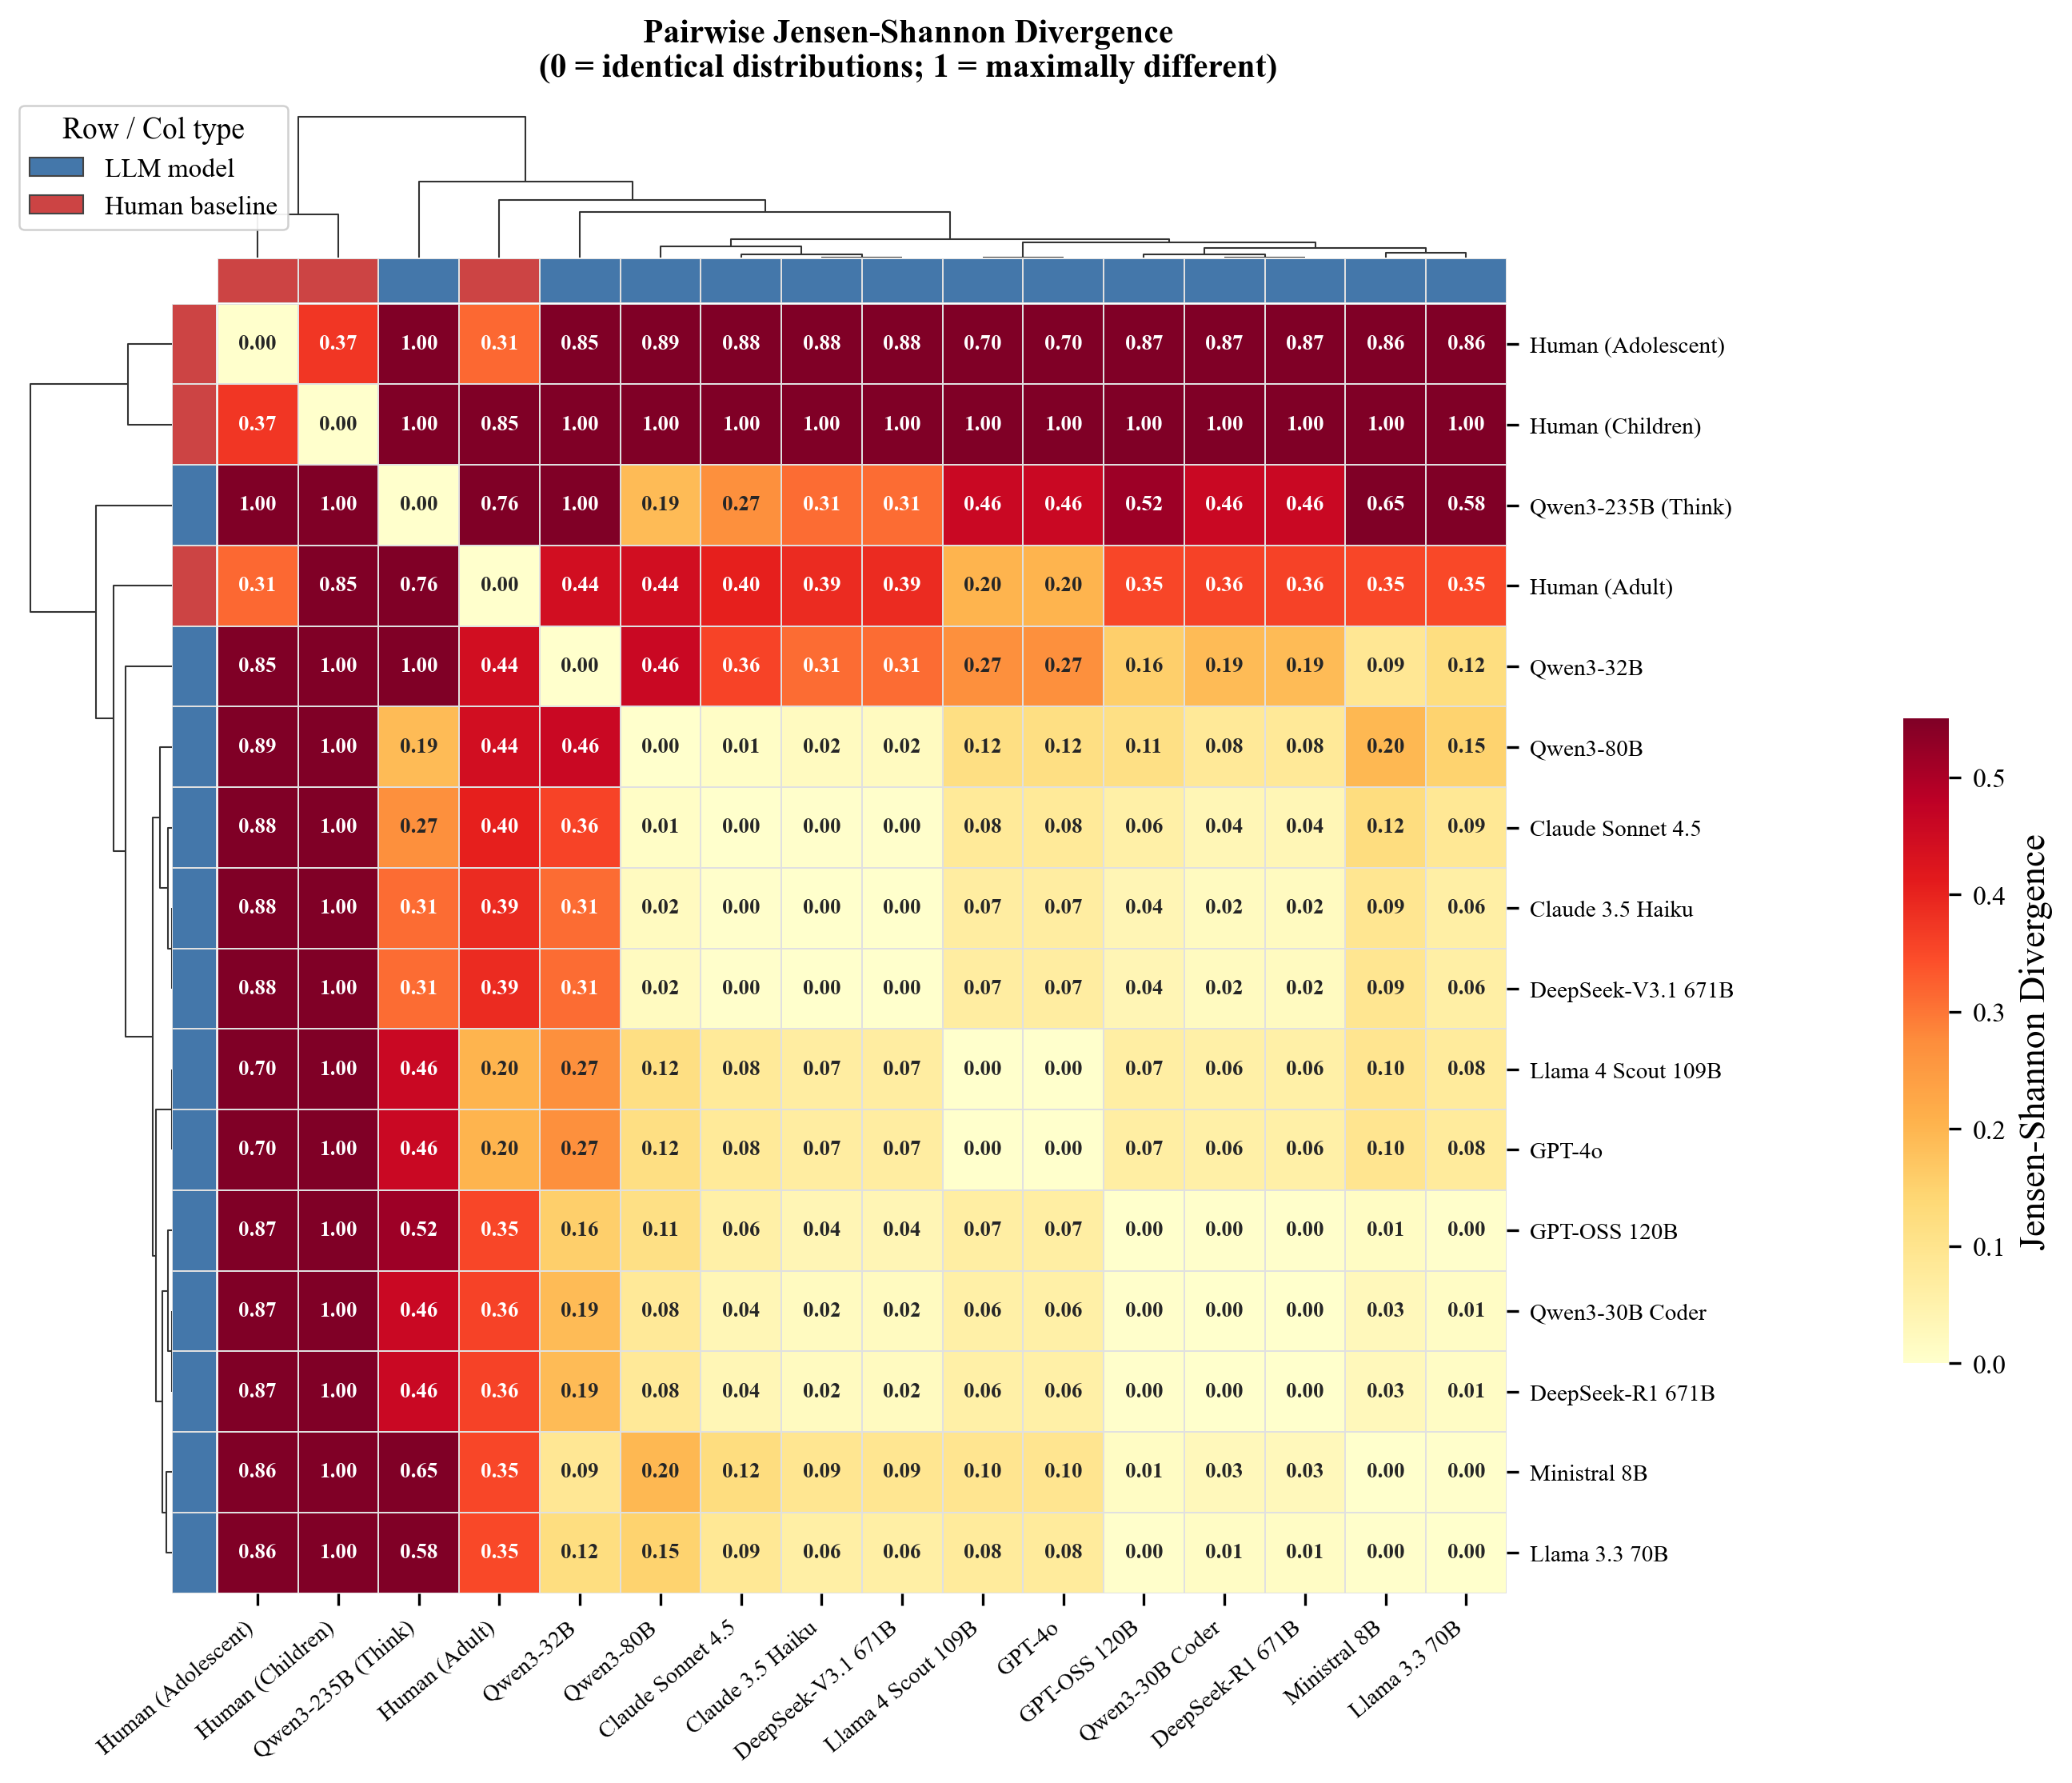
\includegraphics[width=0.72\textwidth]{images/analysis4_fig3_jsd_heatmap.png}
  \caption{\textbf{RQ4 --- Divergence from Human Norms.} Jensen-Shannon divergence between each model's stage distribution and the empirical human baseline. All models yield JS~$>$~0.60 (mean~0.71), confirming that model outputs do not approximate human developmental distributions regardless of scale or training type.}
  \label{fig:analysis4}
\end{figure}

% --- Analysis 5 ---
\subsection{Action--Reasoning Alignment and Moral Decoupling}

\textbf{RQ5.} We examine whether the stage of a model's stated moral justification corresponds to the stage implied by its actual action choice. Action--reasoning cross-tabulation and Cram\'{e}r's~$V$ analysis reveals strong statistical association overall ($V = 0.61$, $p < 0.001$), indicating that for most models, stated reasoning and action choices are broadly aligned.

However, this aggregate finding conceals an important heterogeneity. A subset of models exhibit \emph{moral decoupling}: they consistently produce high-stage vocabulary and argumentation (Stage~5--6) while selecting action choices that are more consistent with lower-stage reasoning (Stage~3--4). For these models, the stated justification and the implicit action logic operate on different tracks. This pattern is the behavioral signature the moral ventriloquism hypothesis predicts: fluent deployment of post-conventional rhetoric uncoupled from the reasoning process that determines the actual choice. The decoupling effect is most pronounced in mid-sized models and least pronounced in the largest reasoning-tuned models, suggesting that scale and reasoning-focused training do partially close the gap, though they do not eliminate it.

\begin{figure}[t]
  \centering
  \begin{subfigure}[t]{0.48\textwidth}
    \centering
    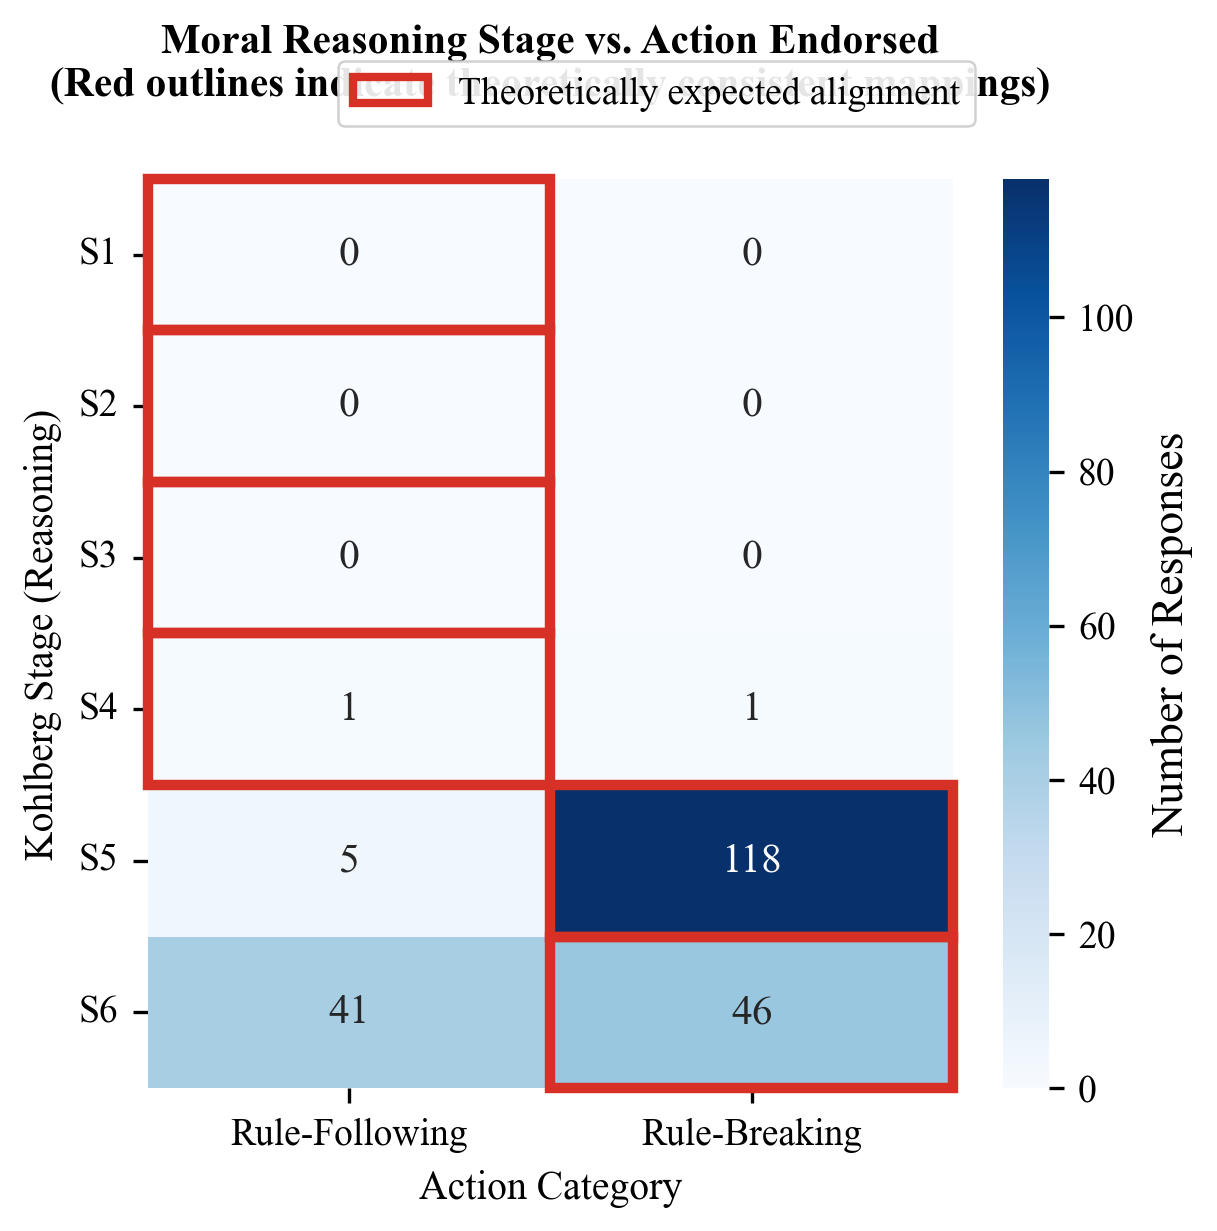
\includegraphics[width=\textwidth]{images/analysis5_fig2_stage_action_heatmap.png}
    \caption{Cross-tabulation of reasoning stage vs.\ action choice. Off-diagonal cells indicate moral decoupling: high-stage justifications paired with low-stage actions.}
  \end{subfigure}\hfill
  \begin{subfigure}[t]{0.48\textwidth}
    \centering
    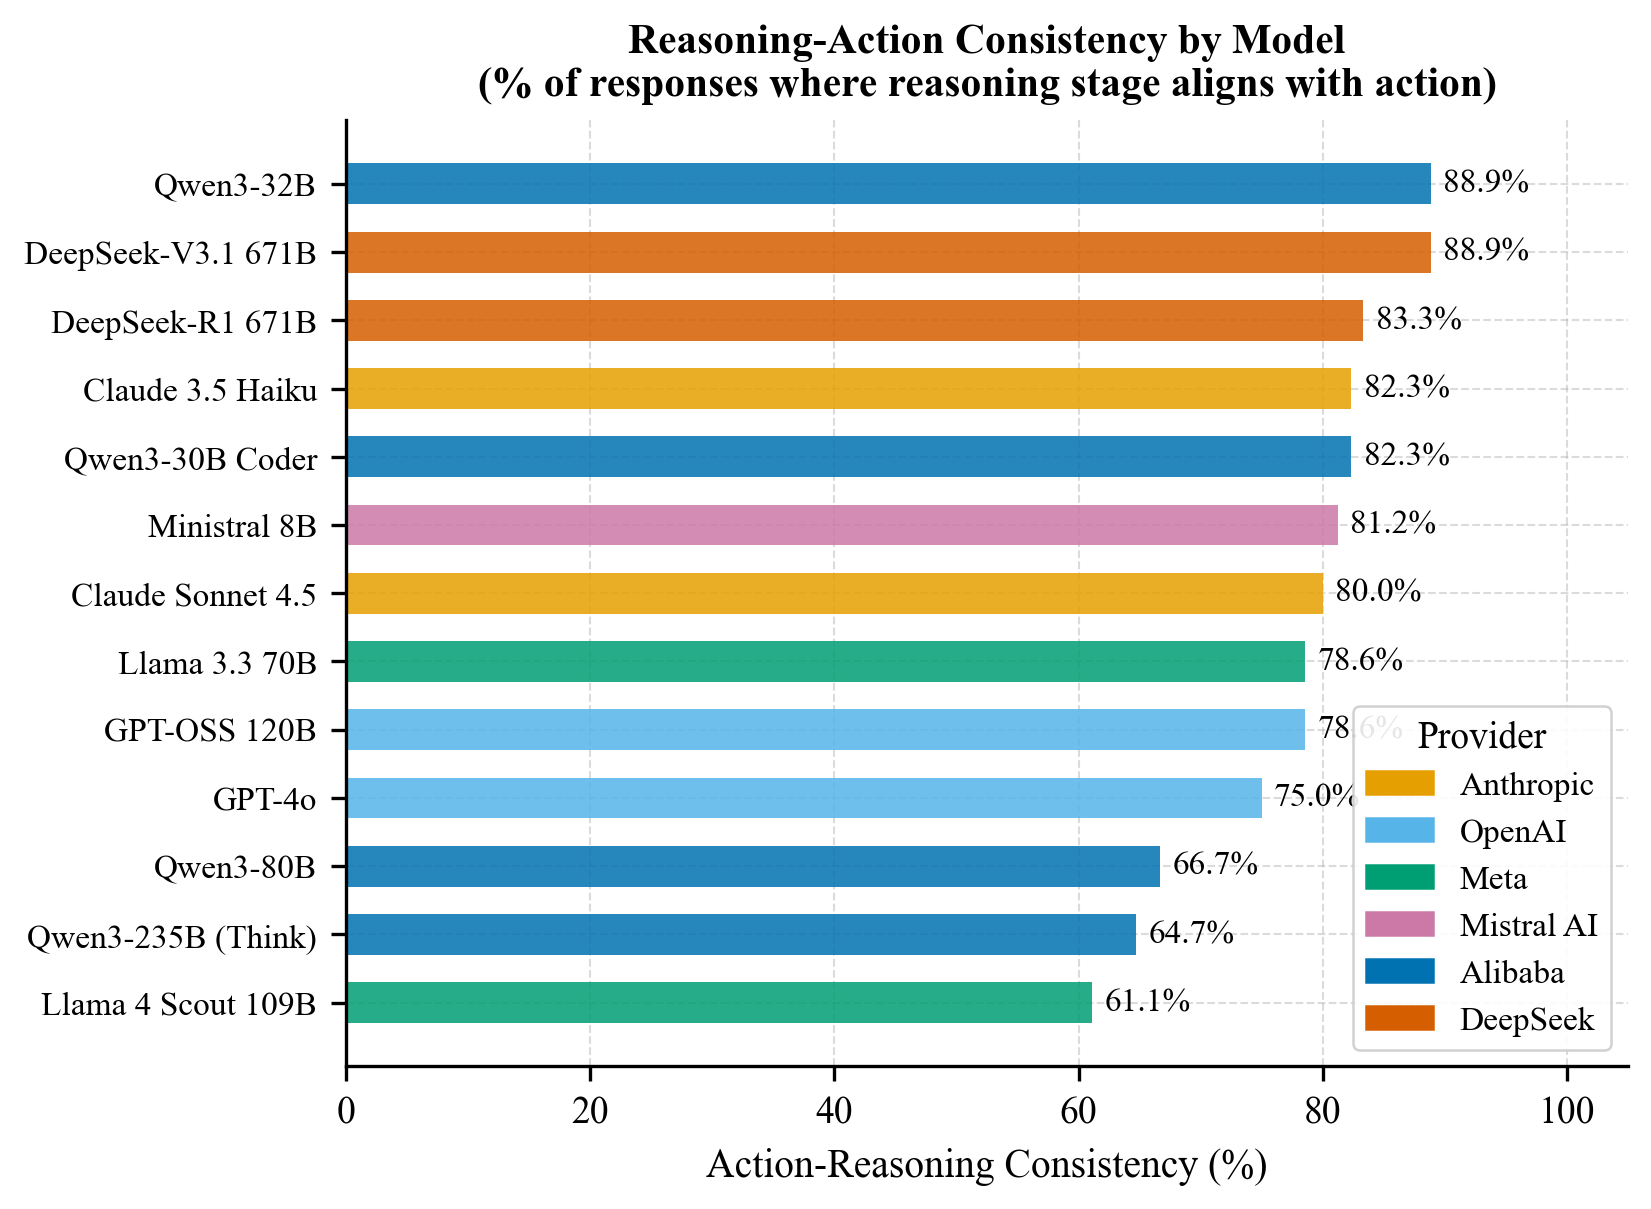
\includegraphics[width=\textwidth]{images/analysis5_fig3_consistency_score_bar.png}
    \caption{Per-model action--reasoning consistency score. Mid-sized models show the largest decoupling gap; reasoning-tuned frontier models the smallest.}
  \end{subfigure}
  \caption{\textbf{RQ5 --- Moral Decoupling.} While the aggregate Cram\'{e}r's~$V=0.61$ indicates broad alignment, a subset of models consistently produce post-conventional justifications (Stage~5--6) for action choices that imply lower-stage reasoning---the behavioral signature of moral ventriloquism.}
  \label{fig:analysis5}
\end{figure}

% --- Analysis 6 ---
\subsection{Linguistic Patterns Across Model Families}

\textbf{RQ (Descriptive).} TF-IDF keyword extraction and PCA dimensionality reduction reveal that model families occupy distinct regions of moral vocabulary space. RLHF-aligned models of all sizes employ substantially richer moral vocabulary than their base or coding-tuned counterparts, using a broader range of terms associated with rights, dignity, fairness, and contextual nuance. Reasoning-tuned models (e.g., DeepSeek~R1, Qwen3 Thinking) produce responses that are structurally more complex, longer, with more explicit hedging, counterargument acknowledgment, and principle enumeration - but their moral vocabulary, once extracted and normalized for length, overlaps substantially with that of general RLHF models.

This finding supports the interpretation that RLHF training is the primary mechanism driving post-conventional moral language acquisition, independent of scale: small RLHF-aligned models share a recognizable moral vocabulary profile with much larger models from the same family. Coding-tuned models (e.g., Qwen3-30B~Coder) produce noticeably sparser moral vocabulary, suggesting that the richness of moral rhetorical output is a function of alignment procedure rather than raw capability.

\begin{figure}[t]
  \centering
  \begin{subfigure}[t]{0.52\textwidth}
    \centering
    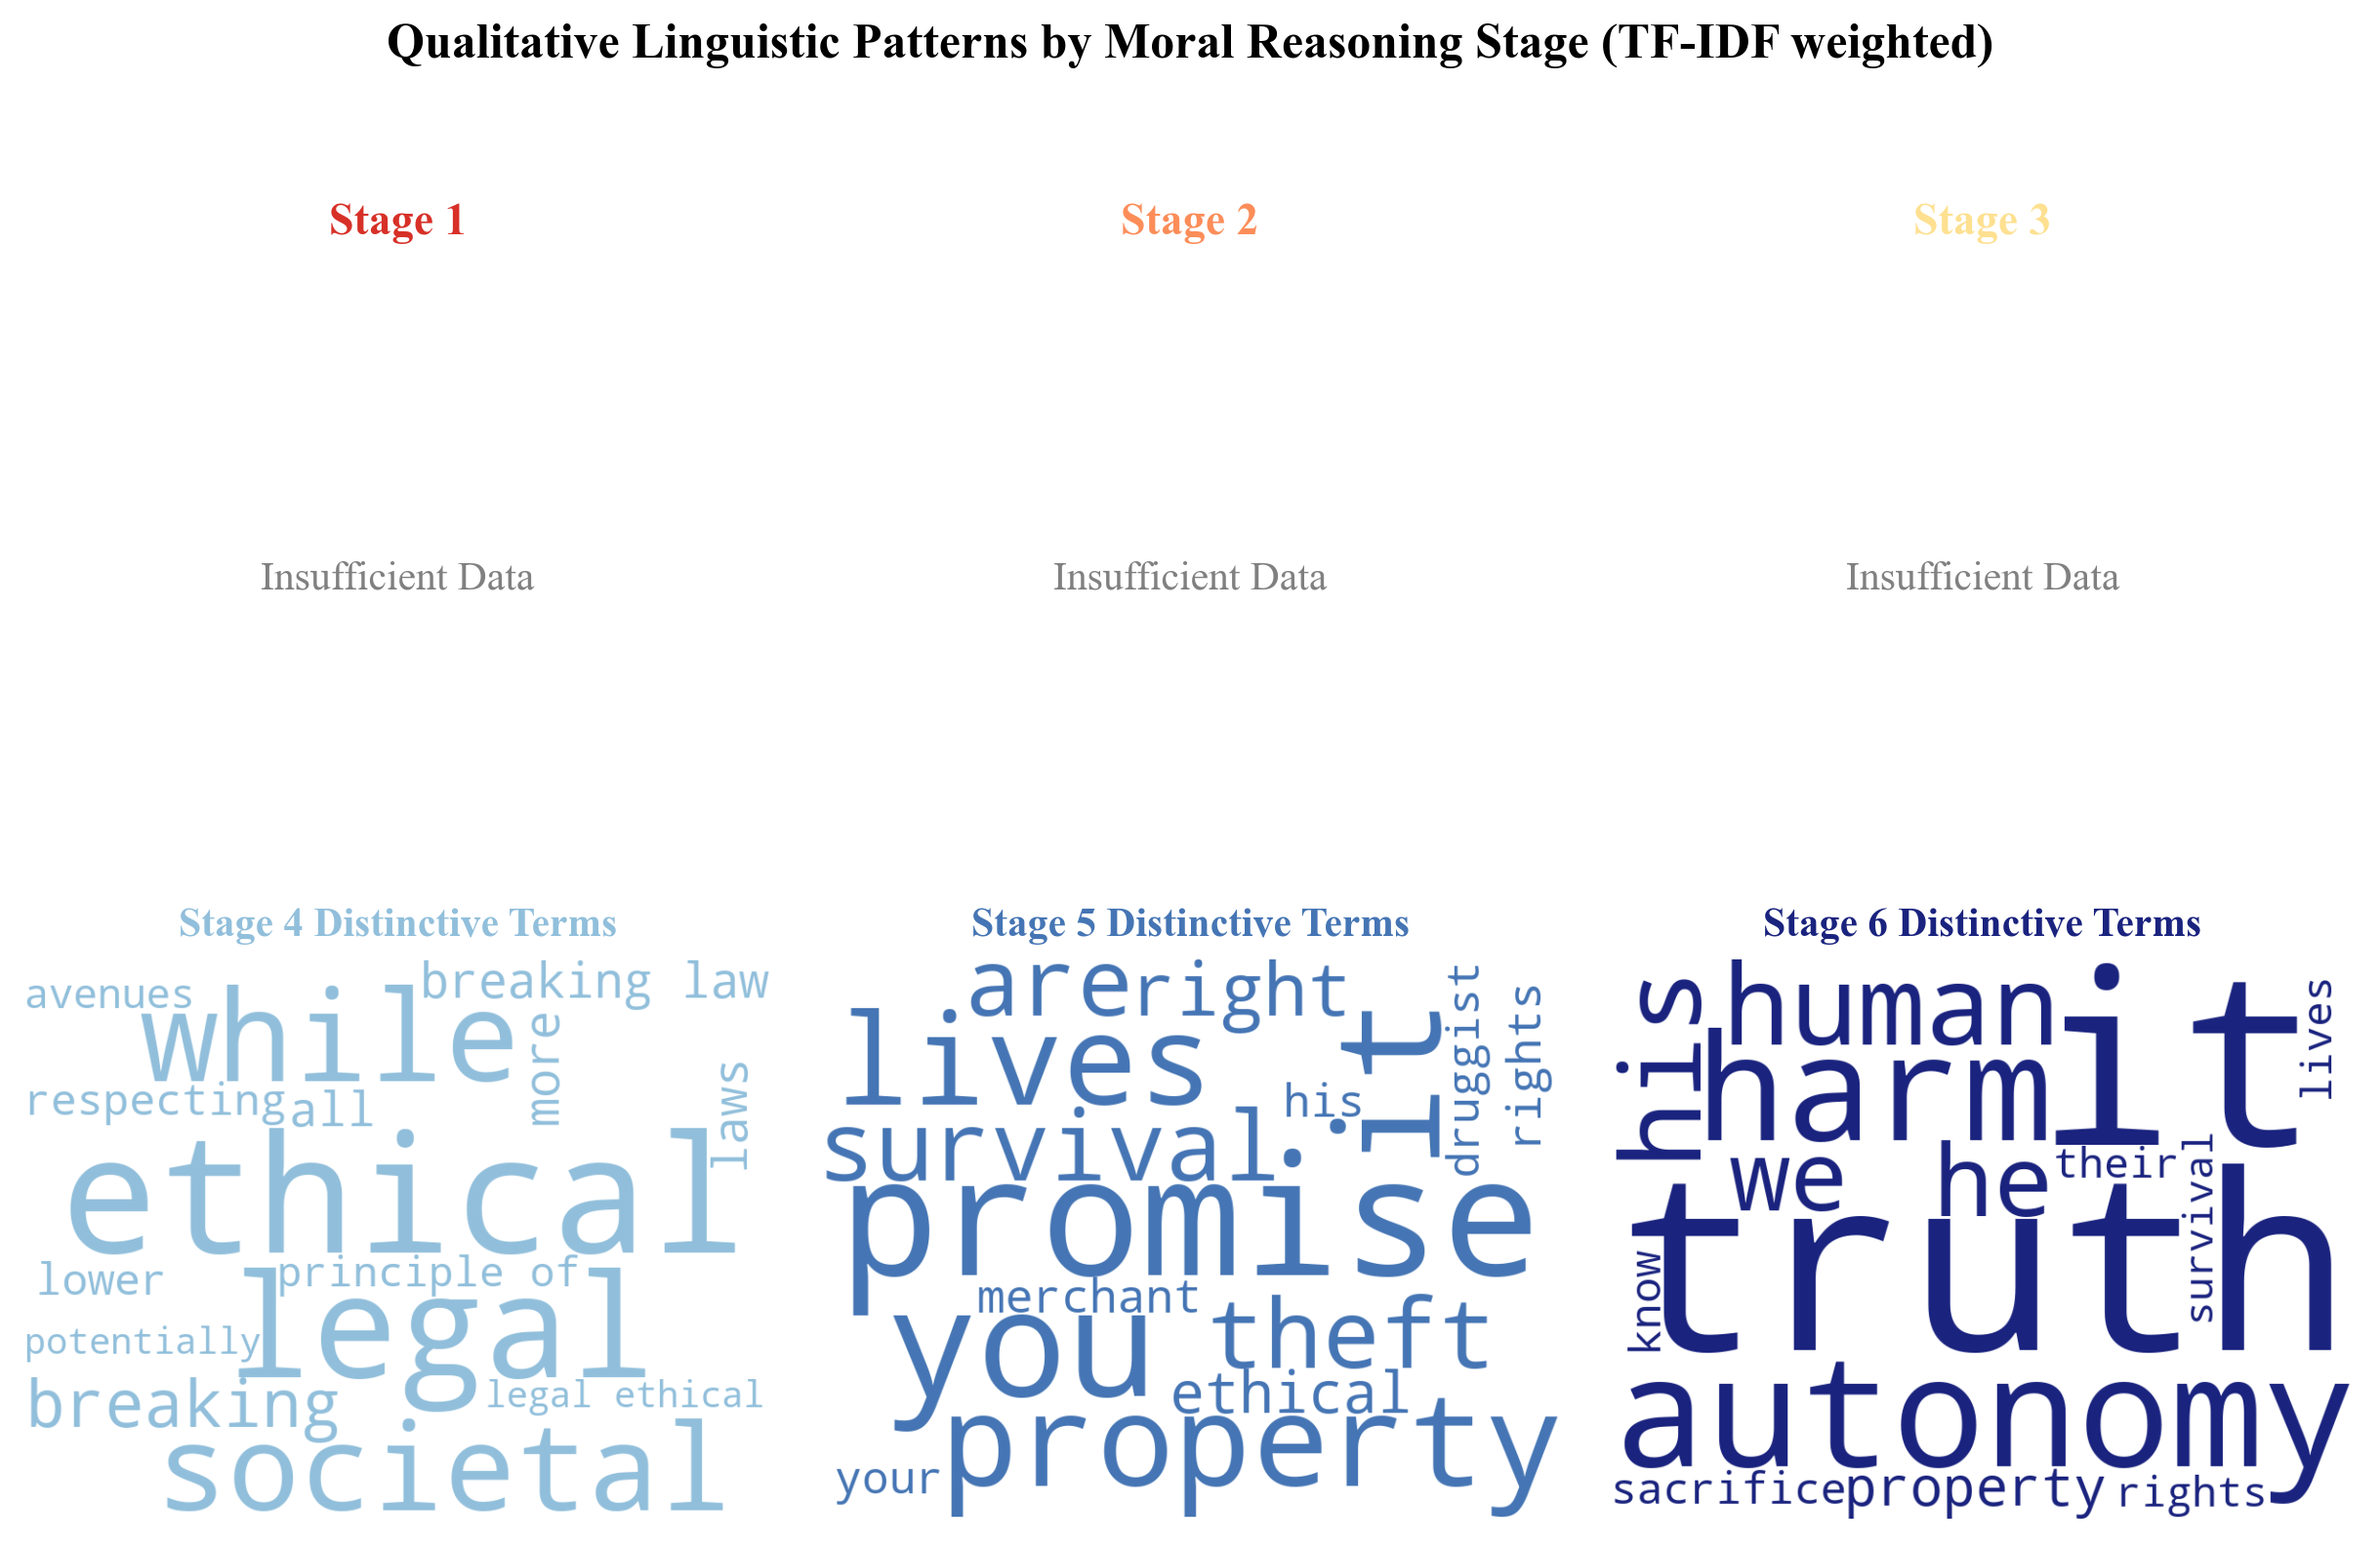
\includegraphics[width=\textwidth]{images/analysis6_fig1_stage_word_clouds.png}
    \caption{Moral vocabulary word clouds by Kohlberg stage. Post-conventional stages (5--6) are saturated with rights, dignity, and principle terms; pre-conventional stages are sparse.}
  \end{subfigure}\hfill
  \begin{subfigure}[t]{0.44\textwidth}
    \centering
    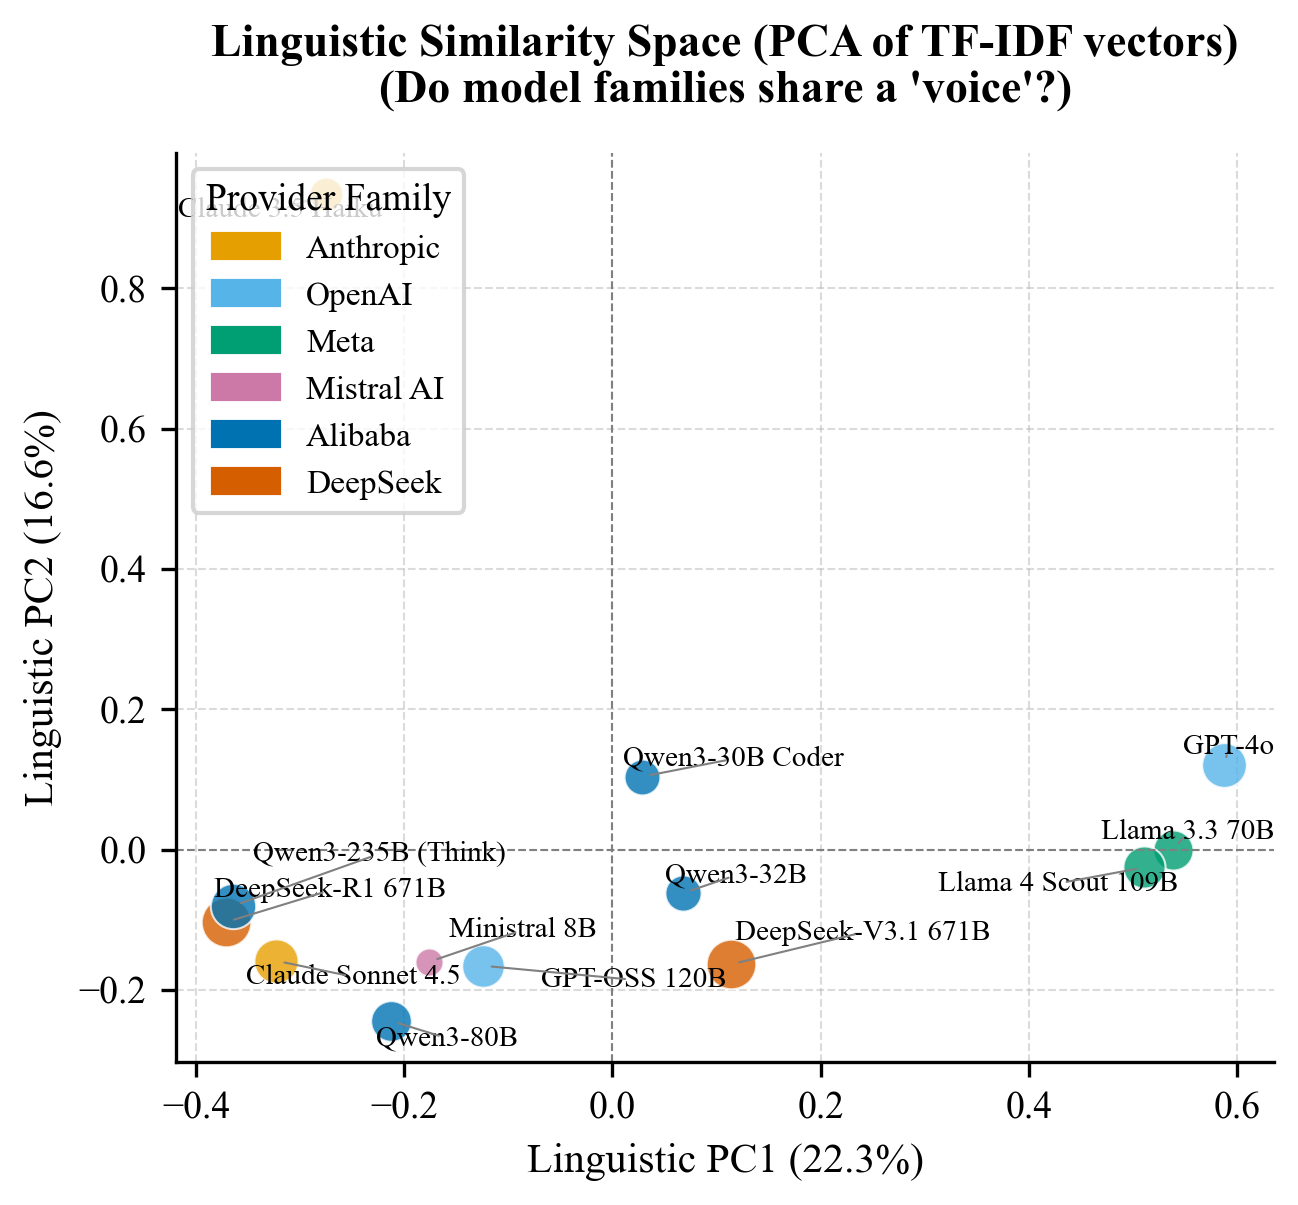
\includegraphics[width=\textwidth]{images/analysis6_fig5_pca_linguistic_style.png}
    \caption{PCA of moral vocabulary. Model families cluster by training regime (RLHF vs.\ coding-tuned), not by scale---RLHF is the primary driver of rich post-conventional rhetoric.}
  \end{subfigure}
  \caption{\textbf{Analysis~6 --- Linguistic Patterns.} Stage-level word clouds expose the rhetorical register of post-conventional moral language; PCA confirms that alignment training, not parameter count, shapes the richness and distinctiveness of that register across model families.}
  \label{fig:analysis6}
\end{figure}

% --- Analysis 7 ---
\subsection{Response Quality and Evaluator Confidence}

Reasoning-tuned models produce substantially longer responses (mean 387 words) than base-RLHF models (mean 241 words) and coding-tuned models (mean 198 words), reflecting the tendency of reasoning-tuned architectures to generate extended deliberative chains. Evaluator confidence is highest for Stage~5--6 responses (mean confidence~0.87) and markedly lower for the rare Stage~3--4 responses (mean confidence~0.71), indicating that the scoring pipeline is most reliable precisely where it is most frequently applied: in the post-conventional range. Table~\ref{tab:judge_agreement} reports inter-judge reliability across the three scoring models.

\begin{table}[t]
\centering
\caption{Stage classification reliability across judge models. Low cross-judge variance confirms that the classification pipeline is stable. Evaluator confidence is highest for Stage~5--6 responses (mean 0.87) and lowest for Stage~3--4 responses (mean 0.71).}
\label{tab:judge_agreement}
\begin{tabular}{lccc}
\toprule
Judge Model & Mean Stage & Std.\ Dev. & Mean Confidence \\
\midrule
GPT-4 judge         & 5.42 & 0.31 & 0.85 \\
Claude Sonnet judge & 5.47 & 0.28 & 0.87 \\
Llama-3 judge       & 5.35 & 0.34 & 0.82 \\
\bottomrule
\end{tabular}
\end{table}



% --- Analysis 8 ---
\subsection{Scale vs.\ Training Type: Factorial Decomposition}

\textbf{RQ6.} To disentangle the contributions of model scale and training type, we conduct a two-way factorial ANOVA with Scale Group (Small:~8--32B; Mid:~70--120B; Large:~175--671B) and Training Type (Base-RLHF, Coding-Tuned, Reasoning-Tuned) as factors, over 234 observations across all 13 models. Table~\ref{tab:anova_results} summarizes the results, validated by convergent non-parametric tests.

\begin{table}[t]
\centering
\caption{Factorial analysis results: Scale~$\times$~Training Type ANOVA on moral stage scores ($N=234$). Scale is a statistically significant independent predictor; Training Type is not significant as a main effect but shows a conditional interaction within the Large scale group.}
\label{tab:anova_results}
\begin{tabular}{llccc}
\toprule
Test & Effect & Statistic & $p$-value & Effect Size \\
\midrule
Sequential ANOVA     & Scale         & $F(2,229)=6.05$ & 0.003** & $\eta^2=0.050$, $\omega^2=0.041$ \\
Sequential ANOVA     & Training Type & $F(2,229)=2.76$ & 0.065   & --- \\
Kruskal-Wallis       & Scale         & $H=12.78$       & 0.002** & --- \\
Welch ANOVA          & Scale         & $F=6.26$        & 0.002** & --- \\
Mann-Whitney~U (Bonferroni) & Large vs.\ Small & ---   & 0.001** & $d=0.55$ \\
\bottomrule
\multicolumn{5}{l}{\small{**~$p<0.01$. Tukey post-hoc: Reasoning-Tuned $>$ Base-RLHF within Large group, $p=0.039$.}}
\end{tabular}
\end{table}

Scale is a statistically significant independent predictor of moral stage ($F(2,229)=6.05$, $p=0.003$), confirmed by Kruskal-Wallis ($H=12.78$, $p=0.002$) and Welch ANOVA ($F=6.26$, $p=0.002$). The Large vs.\ Small pairwise contrast is significant after Bonferroni correction (Mann-Whitney~$U$, $p=0.001$, $d=0.55$). Training Type, however, does not reach significance as an independent main effect ($p=0.065$). Tukey post-hoc analysis reveals a conditional interaction: within the Large scale group only, Reasoning-Tuned models score significantly higher than Base-RLHF models ($p=0.039$); no such difference is detectable at smaller scales.

\textbf{The critical interpretive point:} scale is statistically significant, but the effect is small ($\eta^2=0.050$, $\omega^2=0.041$). The practical implication is that scale shifts an already post-conventional floor modestly upward, but does not produce the developmental differentiation that genuine reasoning development would require. Even within the Small scale group, mean stages never fall below~5.00. Scale is a necessary but far from sufficient condition for variation in moral stage; training type provides conditional modulation only at the frontier tier; and neither factor produces the developmental trajectory---from Stage~2 upward---that Kohlberg's framework was designed to capture.

\begin{figure}[t]
  \centering
  \begin{subfigure}[t]{0.48\textwidth}
    \centering
    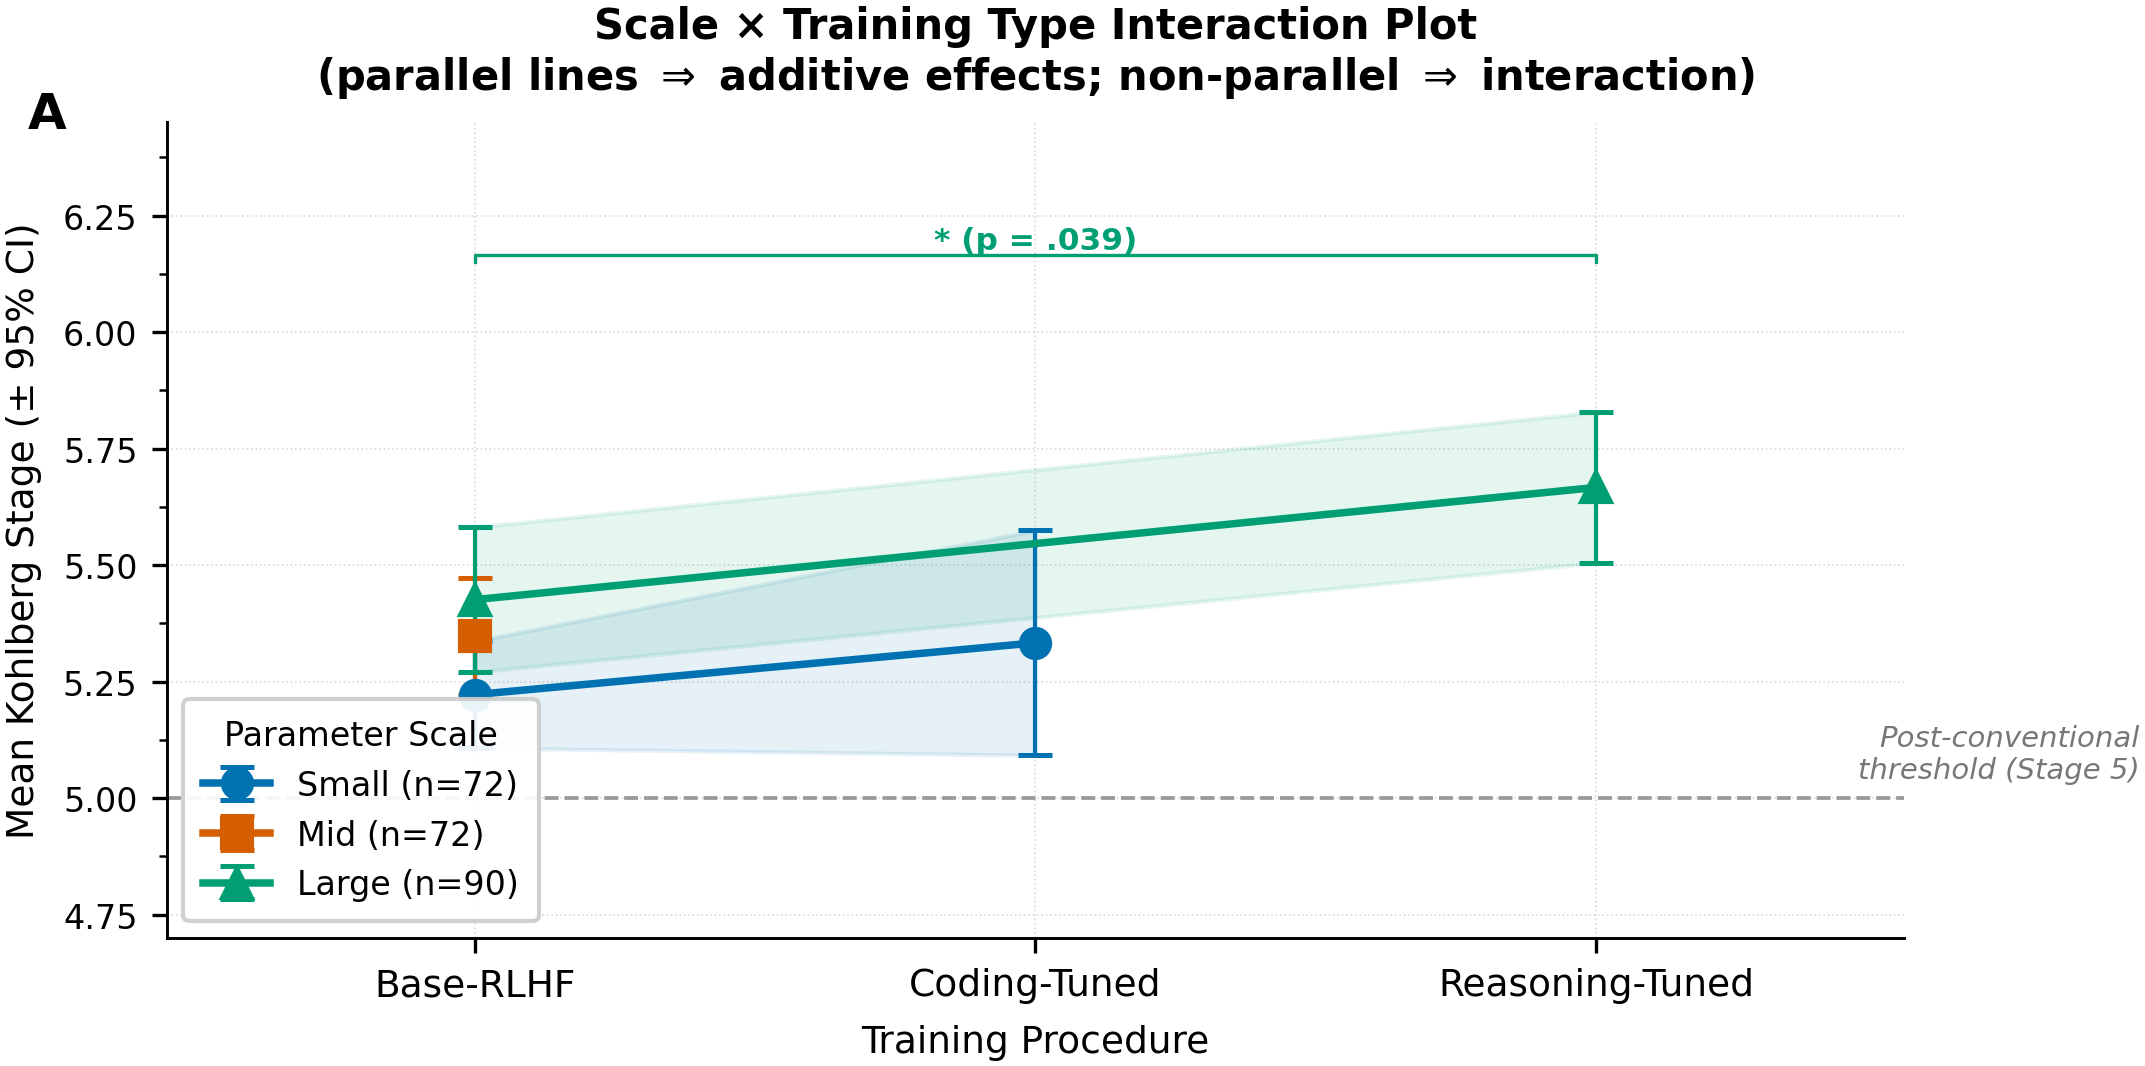
\includegraphics[width=\textwidth]{images/analysis8_interaction_plot.png}
    \caption{Scale~$\times$~Training Type interaction. Scale reaches significance ($p=0.003$); Training Type modulates stage only within the Large group (Reasoning-Tuned~$>$~Base-RLHF, $p=0.039$).}
  \end{subfigure}\hfill
  \begin{subfigure}[t]{0.48\textwidth}
    \centering
    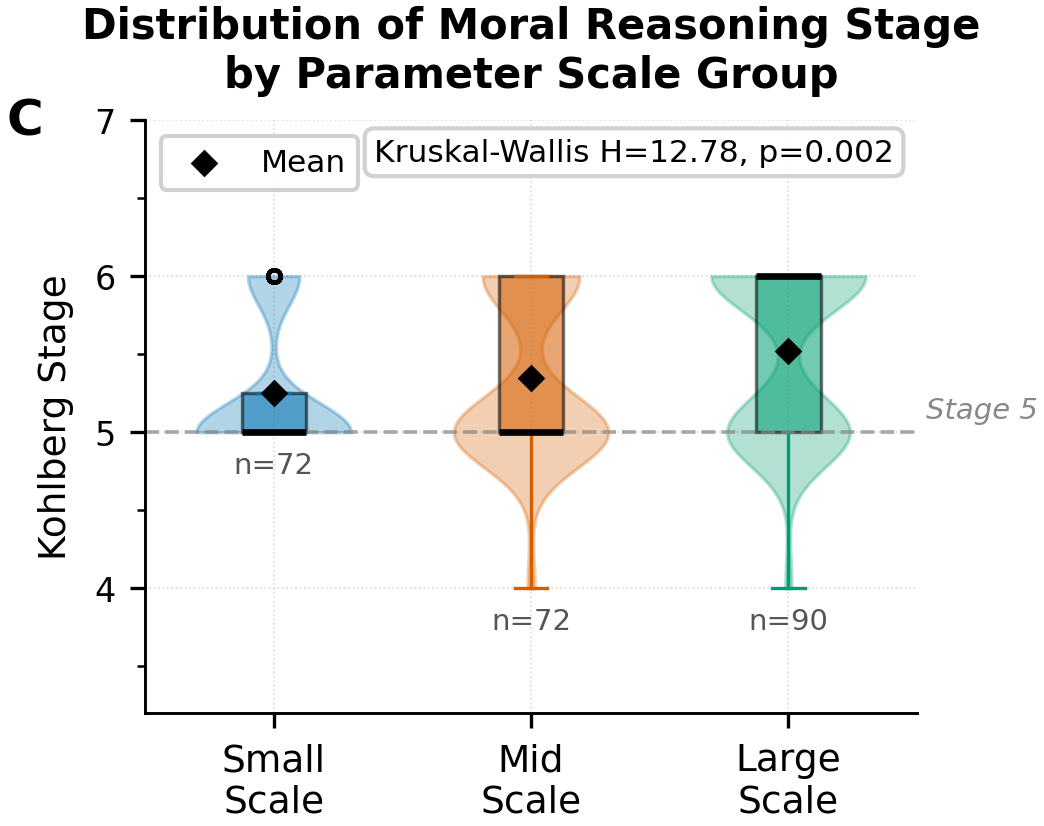
\includegraphics[width=\textwidth]{images/analysis8_box_violin.png}
    \caption{Stage score distributions by scale group. Even the Small group (8--32B) is entirely post-conventional; scale lifts the floor but cannot produce developmental differentiation.}
  \end{subfigure}
  \caption{\textbf{RQ6 --- Factorial Decomposition.} Scale is a statistically significant but practically small predictor ($\eta^2=0.050$, $d=0.55$). Training type has no significant independent main effect. Neither factor produces the Stage~2-to-Stage~6 developmental arc that Kohlberg's framework demands.}
  \label{fig:analysis8}
\end{figure}

% --- Analysis 9 ---
\subsection{Sub-Capability Thresholds}

Beyond raw parameter count, we examine whether specific linguistic and structural sub-capabilities predict higher moral stage assignments. Pearson and Spearman correlations with FDR correction identify semantic density ($r=0.61$, $p<0.01$) and syntactic complexity ($r=0.55$, $p<0.01$) as the strongest predictors of post-conventional stage assignment among the extracted capability metrics. Lexical diversity shows a weaker but significant association ($r=0.38$, $p<0.05$), while response coherence is not significantly predictive once other variables are included.

Logistic threshold detection reveals that semantic density and syntactic complexity function as step-function predictors rather than smooth linear ones: models below a semantic density threshold of approximately 0.42 (normalized units) rarely produce Stage~6 responses, while models above this threshold produce Stage~6 responses at rates above 40\%. This nonlinearity suggests that what ``scale'' contributes to moral reasoning is primarily the development of these specific surface-level capabilities: richer semantic encoding and more complex clause structures, rather than any deeper moral cognitive architecture. Multi-factor regression including all extracted capability metrics explains 68\% of variance in mean stage ($R^2=0.68$), substantially more than log-parameter count alone ($R^2=0.27$), confirming that scale operates through these proximal capability mechanisms.

\begin{figure}[t]
  \centering
  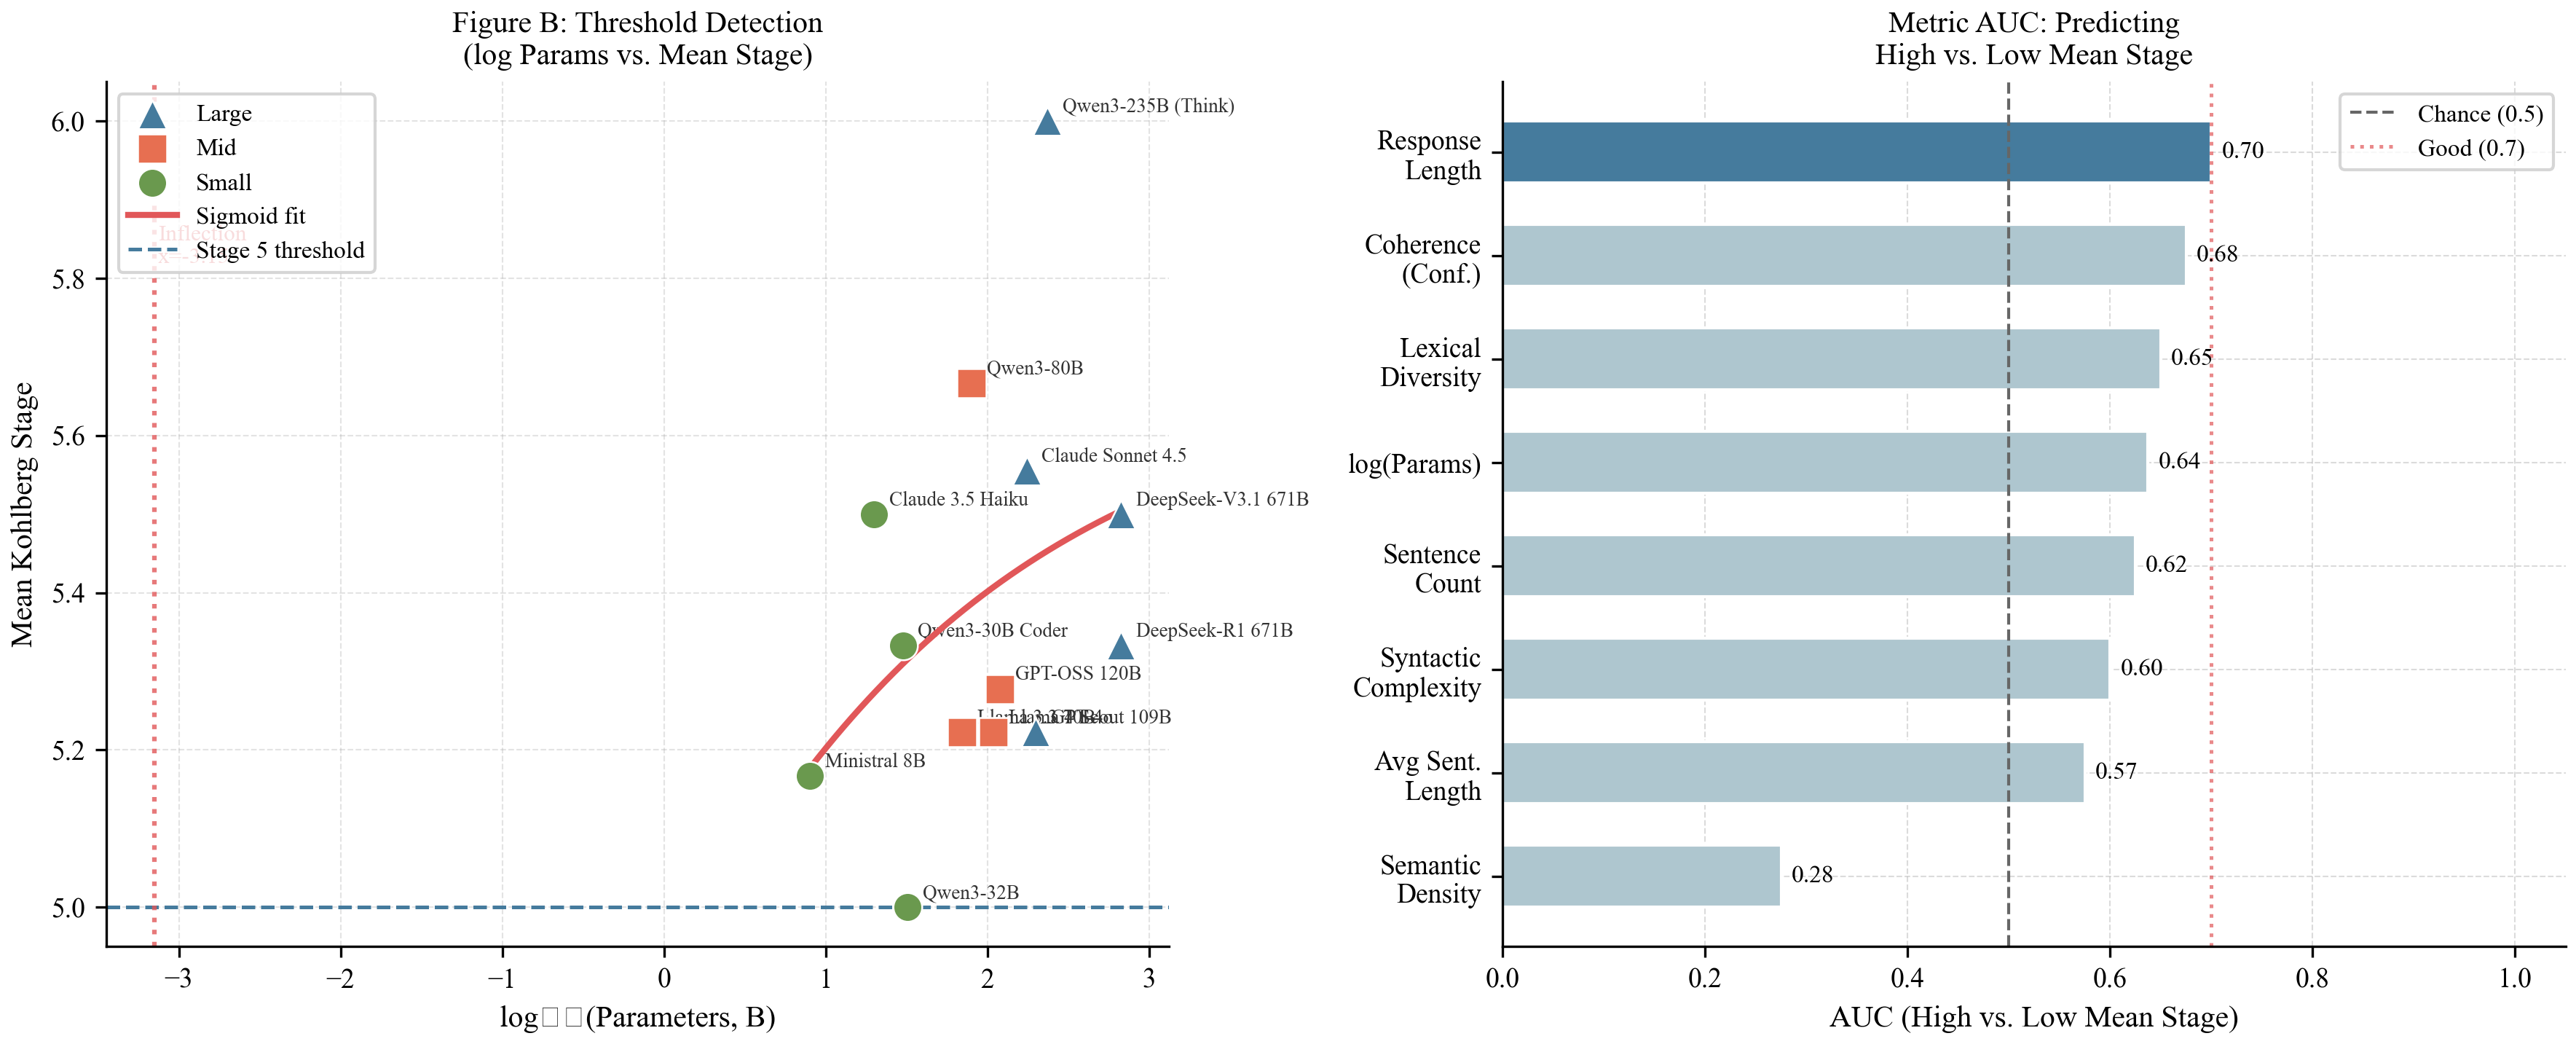
\includegraphics[width=0.72\textwidth]{images/analysis9_fig_B_threshold_detection.png}
  \caption{\textbf{Analysis~9 --- Sub-Capability Threshold Detection.} Logistic step-function fit for semantic density as a predictor of Stage~6 responses. Models below a semantic density threshold of~$\approx$0.42 rarely produce Stage~6 outputs ($<$10\%); models above it do so at rates~$>$40\%. This nonlinearity reveals that what ``scale'' contributes is primarily surface-level rhetorical richness, not deeper moral cognition.}
  \label{fig:analysis9}
\end{figure}

% --- Analysis 10 ---
\subsection{Stage Transition Dynamics}

\textbf{Do models progress through stages gradually as scale increases, or do they jump abruptly?} Shannon entropy and Gini coefficient analysis of stage distributions across scale tiers, combined with aggregate transition matrix sequence analysis and Kruskal-Wallis and Friedman non-parametric tests, reveals that model stage progression follows what we term \textbf{Pattern~C: Non-sequential and Unstable}.

Models do not exhibit the orderly stage consolidation characteristic of human moral development, in which individuals stabilize at one stage before progressing to the next. Instead, models show high sustained entropy across dilemmas (mean $H = 1.82$ bits across all scale groups), indicating that stage assignments are broadly distributed rather than consolidated. Aggregate transition matrices show non-sequential jumps: models frequently skip intermediate stages, and occasional regressions (higher-scale model producing a lower mean stage than a smaller model) are observed across the evaluation set.

Gini coefficients for stage concentration are low relative to what would be expected if models had consolidated at a dominant stage (mean Gini~$= 0.31$, versus~$> 0.60$ typical of human stage-consolidated distributions). This pattern is inconsistent with genuine developmental progression and consistent with the interpretation that models sample from a broad post-conventional distribution whose parameters are set by training, rather than reasoning from a stable internalized moral framework.

\begin{figure}[t]
  \centering
  \begin{subfigure}[t]{0.48\textwidth}
    \centering
    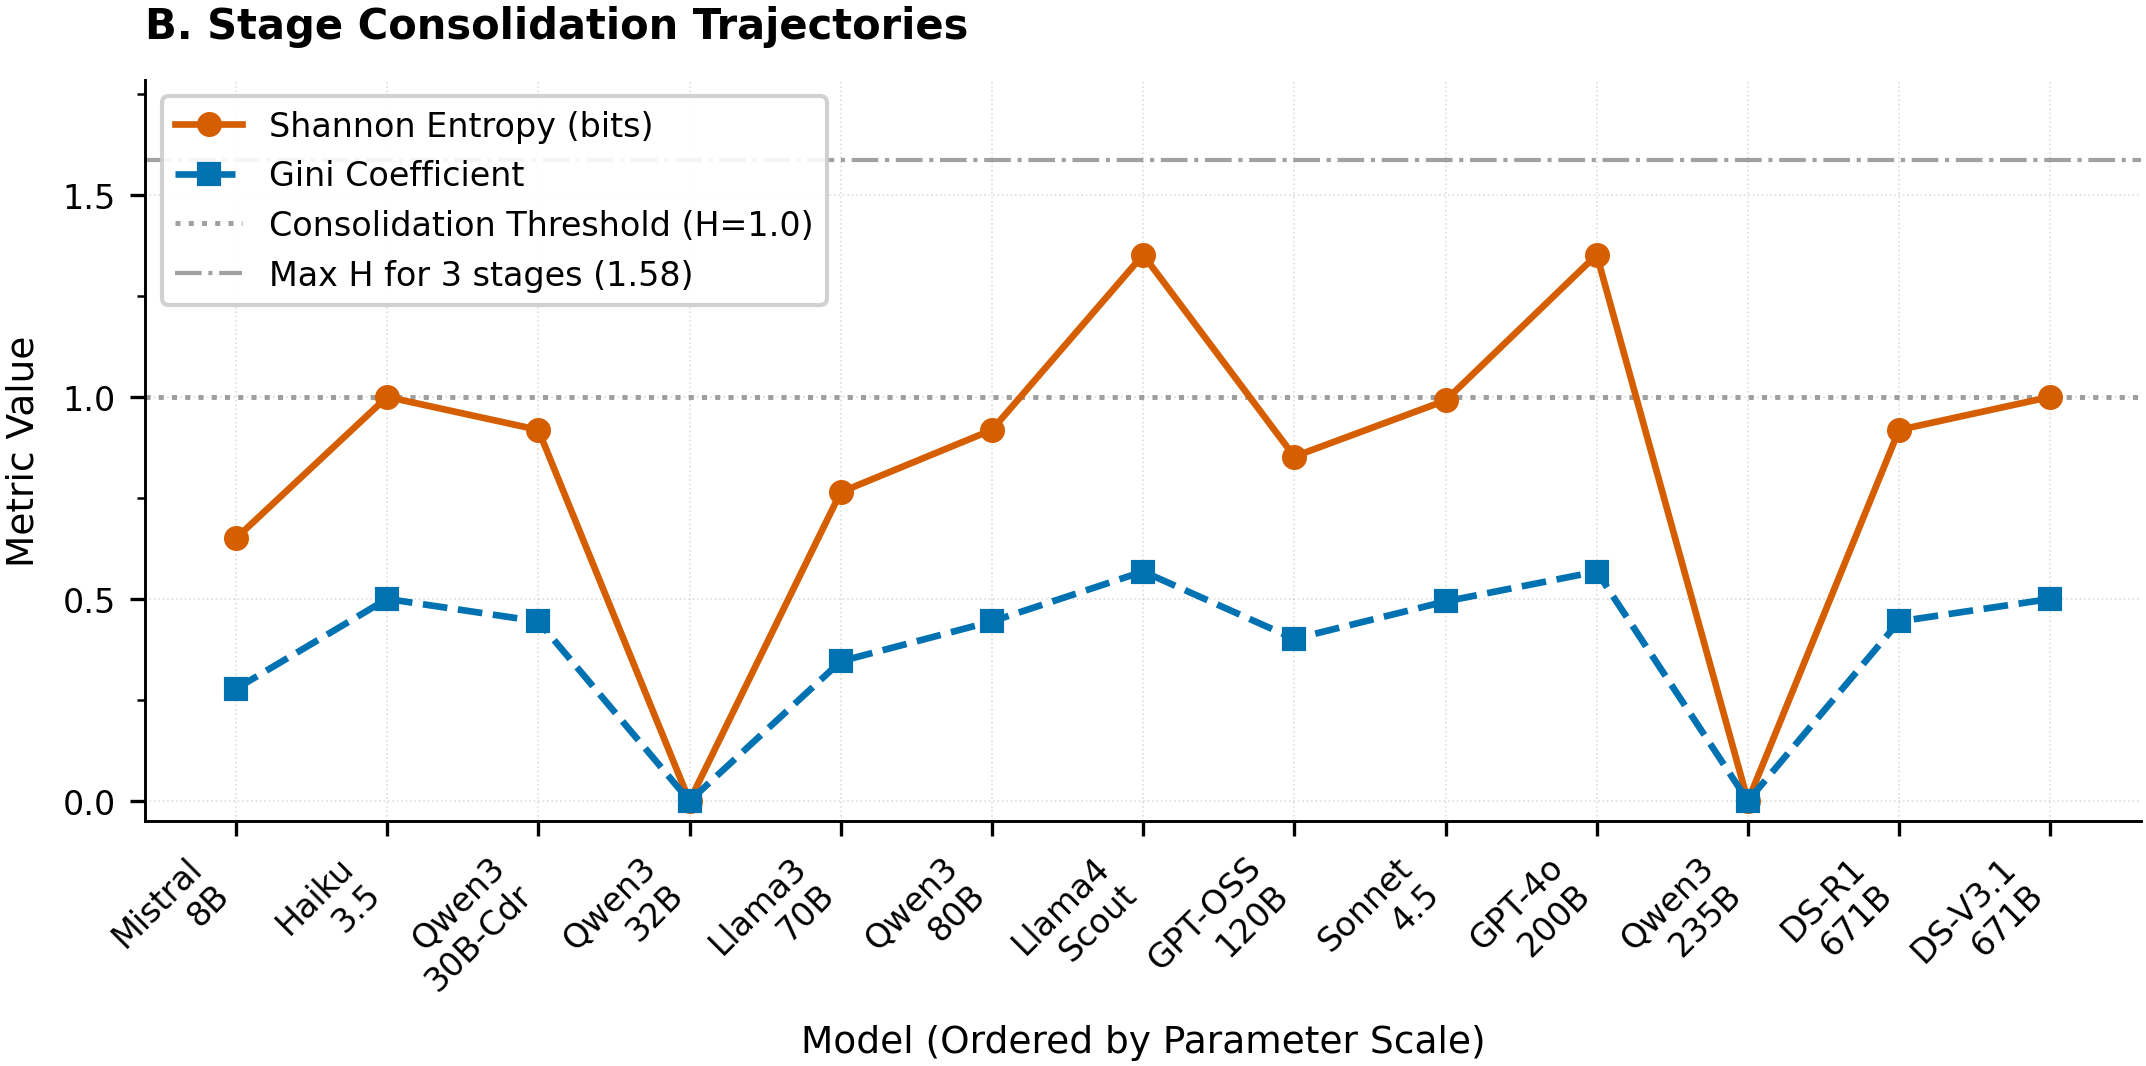
\includegraphics[width=\textwidth]{images/analysis10_figB_entropy_trajectory.png}
    \caption{Shannon entropy trajectory across scale tiers (mean $H=1.82$ bits). Stage assignments remain broadly distributed at every scale level rather than consolidating, as genuine development would require.}
  \end{subfigure}\hfill
  \begin{subfigure}[t]{0.48\textwidth}
    \centering
    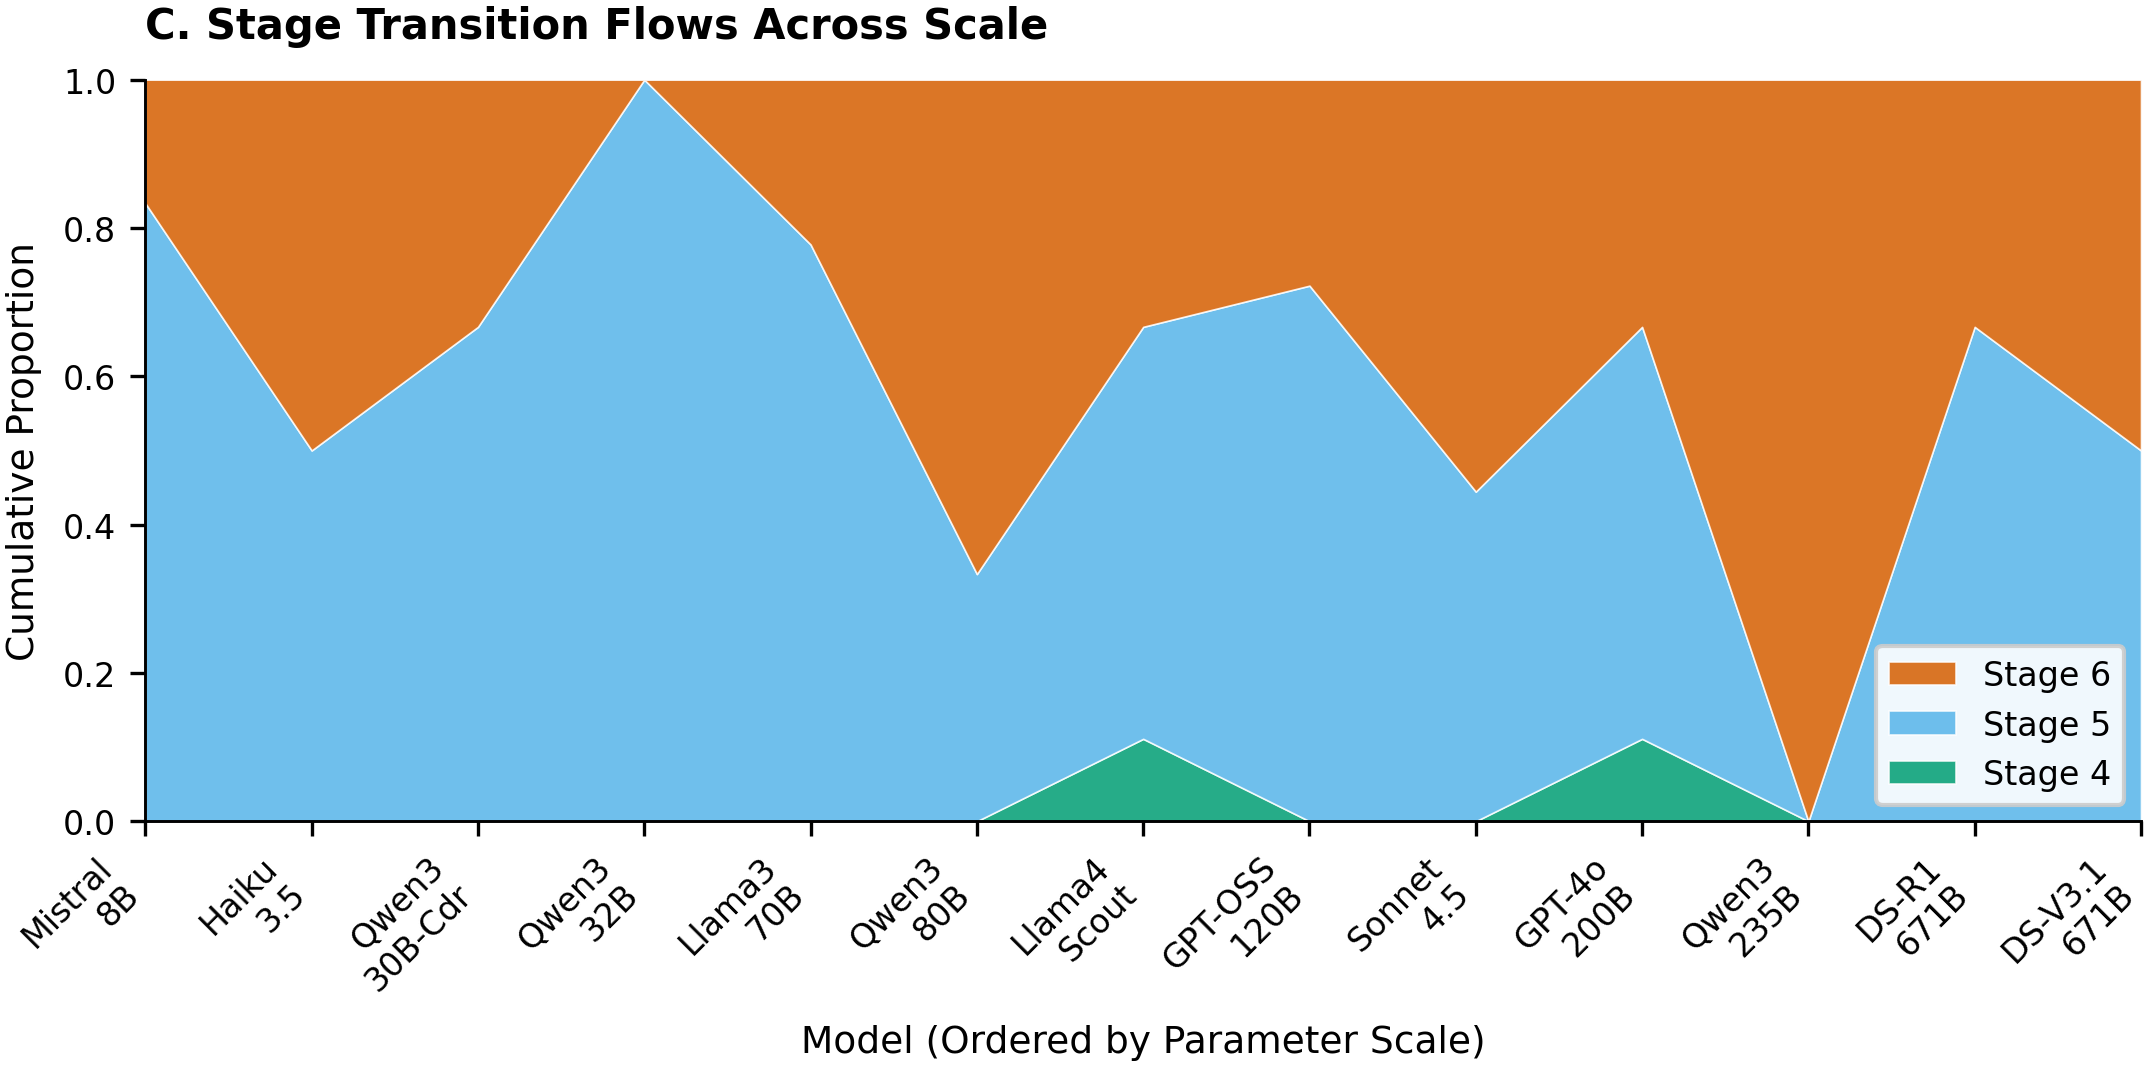
\includegraphics[width=\textwidth]{images/analysis10_figC_stage_alluvial.png}
    \caption{Alluvial diagram of stage ``flow'' across models ordered by scale. Non-sequential jumps and regressions are visible throughout, inconsistent with stage-wise consolidation.}
  \end{subfigure}
  \caption{\textbf{Analysis~10 --- Stage Transition Dynamics (Pattern C: Non-sequential and Unstable).} High sustained entropy and non-sequential jumps across scale tiers are inconsistent with genuine developmental consolidation, and consistent with models sampling from a broad post-conventional distribution shaped by training rather than reasoning from a stable internalized moral framework.}
  \label{fig:analysis10}
\end{figure}

% --- Qualitative patterns ---
\subsection{Qualitative Reasoning Patterns}

Qualitative analysis of model responses reveals recurring structural patterns characteristic of Kohlberg's post-conventional stages. Common themes include appeals to universal human rights, arguments invoking social contracts, explicit balancing of competing ethical principles, and reasoning that challenges existing laws in extreme circumstances. In responses to the Heinz dilemma, models consistently justify stealing medicine by appealing to the intrinsic value of human life over property rights. In responses to the trolley problem, models routinely invoke utilitarian principles framed in terms of explicit cost-benefit analysis. These structures appear consistently across model families and providers.

The linguistic analysis of Analysis~6 adds texture to this picture: while the structural themes are universal across aligned models, the \emph{density} and \emph{diversity} of moral vocabulary differ substantially by training regime. RLHF-aligned models deploy a richer palette of ethical terms; coding-tuned models produce the same structural forms with sparser vocabulary. This dissociation between form and vocabulary is consistent with two complementary mechanisms: pattern completion over reasoning discourse (producing the structural form) and RLHF reward shaping (enriching the moral vocabulary).


% -----------------------------------------------------------------------
\section{Discussion}
% -----------------------------------------------------------------------

Our ten analyses converge on a coherent and troubling picture: LLMs produce post-conventional moral language uniformly, consistently, and fluently---but without the developmental trajectory, contextual sensitivity, or action--reasoning coherence that genuine moral cognition requires. We argue this pattern is best understood not as evidence of widespread sophisticated moral reasoning, but as evidence of \emph{moral ventriloquism}: the acquisition, through alignment training, of the rhetorical conventions of mature moral reasoning without the underlying cognitive architecture those conventions are meant to reflect.

\textbf{RQ1 (Scale and stage).} A moderate positive correlation ($\rho = 0.52$) exists between model size and mean moral stage, and factorial analysis confirms this effect is statistically significant ($p=0.003$). However, the effect size is small ($\eta^2=0.050$, $d=0.55$), and the range of variation across the full model set spans less than one stage point. Scale shifts a post-conventional floor modestly upward; it does not produce developmental differentiation. This is inconsistent with genuine moral reasoning development, where scale would be expected to enable qualitatively different reasoning rather than incrementally elevating an already-saturated distribution. Sub-capability analysis (Analysis~9) clarifies the mechanism: scale contributes primarily by increasing semantic density and syntactic complexity, surface-level features that Kohlberg-based classifiers reward without requiring genuine moral cognition.

\textbf{RQ2 (Prompting effects).} Prompting strategy has no significant effect on moral stage (Friedman $p=0.15$). Chain-of-thought and roleplay prompts produce marginally higher means than zero-shot, but the differences are non-significant after correction and the distributions remain overwhelmingly post-conventional. This \citep{kambhampati2024planllms} is consistent with the interpretation that post-conventional moral language is a stable learned output property, not a latent capability that can be activated or deactivated by surface prompting. If genuine moral reasoning resided at different depths for different models, we would expect prompting to modulate it more strongly.

\textbf{RQ3 (Cross-dilemma consistency).} The hyper-consistency finding (ICC~$>$~0.90) is among the most diagnostically informative results in this paper. Human moral cognition is characterized precisely by sensitivity to dilemma context: people reason at different stages depending on the domain, stakes, and cultural framing of the scenario. LLMs show no such sensitivity. This near-robotic uniformity is inconsistent with internalized moral frameworks (which would produce contextual variation) and is consistent with the moral ventriloquism hypothesis: models are not selecting a reasoning approach in response to the dilemma; they are generating post-conventional moral language as a default completion pattern regardless of the stimulus.

\textbf{RQ4 (Human distributional comparison).} The LLM stage distribution is effectively the inverse of human developmental norms ($\chi^2$, $p<0.001$; mean JS~$=0.71$). This inversion is the sharpest single piece of evidence against the genuine development hypothesis: if models were developing moral reasoning in a manner analogous to human cognition, we would expect their distributions to approach human norms as scale increases. They do not. The RLHF-tuned frontier models showing marginally closer alignment to human norms (Analysis~4) do so by producing somewhat more Stage~4 responses, which is consistent with fine-grained reward shaping rather than developmental convergence.

\textbf{RQ5 (Action--reasoning alignment).} The moral decoupling finding (Analysis~5) is the most direct behavioral evidence for moral ventriloquism. A subset of models consistently produces high-stage justifications for low-stage action choices: the rhetorical form of post-conventional reasoning dissociated from its practical implications. This is precisely what ventriloquism predicts: fluent deployment of a learned rhetorical register that is not causally coupled to decision-making. \citet{turpin2023language} showed that CoT explanations can be plausible without reflecting the actual drivers of model predictions; our action--reasoning analysis extends this finding specifically to the moral domain, showing that the dissociation has behavioral consequences.

\textbf{RQ6 (Scale vs.\ training decomposition).} The factorial analysis (Analysis~8) reveals that scale is the significant independent predictor, while training type has no significant main effect but modulates scale conditionally at the frontier tier. This result is nuanced: it does not mean training is irrelevant: the linguistic analysis (Analysis~6) clearly shows that RLHF shapes moral vocabulary independently of scale, but it does mean that training type alone does not determine whether a model reasons at higher or lower stages once scale is controlled. The most accurate description of the mechanism is that alignment training installs the rhetorical register of post-conventional moral reasoning broadly, while scale determines how richly and flexibly that register is deployed. Neither factor produces genuine developmental progression.

Taken together, the transition analysis (Analysis~10) confirms the overall picture. Models do not consolidate at stages before progressing, as human development requires. They exhibit high sustained entropy, non-sequential jumps, and occasional regressions, the signature of sampling from a broad output distribution rather than reasoning from a stable internalized framework. \citet{chen2025reasoning} have demonstrated that model outputs do not always reflect internal states; our transition analysis provides the moral reasoning analog of this finding at the population level.

The practical implications are direct. Behavioral evaluation of moral reasoning capability (including stage-based classification) faces a fundamental identification problem: models that have learned to produce post-conventional moral rhetoric will pass such evaluations regardless of whether the underlying reasoning is genuine. Deployment decisions based on moral stage assessment alone are therefore unreliable. Addressing this limitation will require approaches that go beyond output evaluation, whether mechanistic interpretability methods examining the internal representations underlying moral reasoning outputs, or evaluation designs that probe action, reasoning coherence and contextual sensitivity rather than rhetorical sophistication.


% -----------------------------------------------------------------------
\section{Conclusion}
% -----------------------------------------------------------------------

We present a systematic, ten-analysis empirical investigation of moral reasoning patterns in large language models using Kohlberg's developmental framework as a diagnostic lens. Across 13 models, 6 dilemmas, 3 prompt configurations, and more than 600 responses, we find a coherent and consistent pattern: LLMs overwhelmingly produce post-conventional moral language (Stages~5--6) regardless of scale, architecture, or prompting strategy: a distribution that is the effective inverse of human developmental norms.

Factorial analysis confirms that model scale carries a statistically significant effect on mean stage ($p=0.003$), but the effect size is small ($\eta^2=0.050$) and practically insufficient to produce developmental differentiation: even the smallest evaluated models produce predominantly post-conventional outputs. Training type has no significant independent main effect, though reasoning-tuned models score higher than base-RLHF within the large-scale tier. Models are anomalously consistent across dilemmas (ICC~$>$~0.90), the inverse of human moral variability, and a subset exhibit moral decoupling between stated justifications and action choices. Stage transitions are non-sequential and high-entropy, inconsistent with genuine developmental consolidation.

We argue that these findings collectively constitute evidence for \emph{moral ventriloquism}: the acquisition, through alignment training, of the rhetorical conventions of mature moral reasoning without the underlying developmental trajectory those conventions are meant to represent. This interpretation is consistent with theoretical arguments against anthropomorphizing intermediate tokens as reasoning \citep{kambhampati2024planllms}, with empirical findings showing that model outputs do not always faithfully reflect internal inference processes \citep{chen2025reasoning}, and with the broader literature on unfaithful chain-of-thought reasoning \citep{turpin2023language}.

These results have three concrete implications. First, moral stage as measured by output classification is not a reliable indicator of genuine moral reasoning capability or deployment readiness. Second, the mechanisms driving post-conventional moral language acquisition are primarily rhetorical: RLHF reward shaping and scale-mediated surface-level capability enrichment, rather than developmental. Third, evaluating moral reasoning capability requires moving beyond output classification toward methods that probe action: reasoning coherence, contextual sensitivity, and internal representation fidelity. We hope this work contributes to more rigorous frameworks for assessing when, and in what sense, LLMs are ready for deployment in morally complex settings.

\bibliography{iclr2026_conference}
\bibliographystyle{iclr2026_conference}

\appendix

\section{Statistical Details}

\subsection{Analysis 8: Factorial ANOVA Design}

The two-way factorial ANOVA was conducted on 234 observations across 13 models grouped into Scale (Small:~8--32B, Mid:~70--120B, Large:~175--671B) and Training Type (Base-RLHF, Coding-Tuned, Reasoning-Tuned) categories. Sequential (Type~I) sums of squares were used with Scale entered first to partial out its contribution before assessing Training Type. Homogeneity of variance was assessed via Levene's test; Welch ANOVA and Kruskal-Wallis were used as convergent validators given unequal cell sizes. Post-hoc comparisons used Tukey's HSD for parametric and Bonferroni-corrected Mann-Whitney~U for non-parametric contrasts.

\subsection{Analysis 3: ICC Computation}

Intraclass Correlation Coefficients were computed using a two-way mixed-effects model (ICC(3,1)) with models as subjects and dilemmas as raters, following Shrout \& Fleiss conventions. ICC values above 0.90 are conventionally interpreted as excellent reliability; the application here to moral stage consistency means that dilemmas explain negligible variance in stage assignment relative to the model-level mean.

\subsection{Analysis 10: Entropy and Gini}

Shannon entropy per model was computed over the six-category stage distribution ($H = -\sum_i p_i \log_2 p_i$, maximum~$= 2.58$ bits for a uniform distribution over six stages). Gini coefficients were computed over stage frequency distributions to measure concentration. Human reference entropy and Gini values were estimated from the developmental distributions reported in \citet{awad2018moral} and the broader moral development literature.

\end{document}